\chapter{Experiments, Results and Discussion}\label{cha:results}

To evaluate the efficacy of the proposed self-healing security framework, a series of experiments were conducted assessing both the edge-layer detection capabilities and the cloud-tier multi-agent remediation performance.

\section{Experimental Setup}

\textbf{Dataset:} The framework's edge-layer detection ensemble and the offline classifier feature schema were both evaluated using the CIC IIoT 2025 dataset (DataSense), a real-time sensor-and-network-traffic benchmark released by the Canadian Institute for Cybersecurity in December 2024 \cite{Firouzi2025}. The full dataset comprises 685{,}671 labelled instances (58.44\% benign, 41.56\% attack) spanning 50 attack types across seven categories (DDoS, DoS, Reconnaissance, Web, Bruteforce, MITM, and Malware/Mirai); the subset used for the preprocessing and evaluation reported in this chapter aggregates traffic into 2-second windows, yielding 113{,}144 records with 94 initial columns, no null values, and no duplicate records (approximately 81.1\,MB in raw form). Figure \ref{fig:class_distribution} shows the resulting class distribution at the 8-category grouping (benign plus the seven attack categories) used for the offline classifier validation in Section \ref{sec:cloud_eval}; as the figure shows, the dataset is substantially imbalanced toward benign traffic, which is why evaluation throughout this chapter reports precision, recall, F1-score, and confusion matrices rather than accuracy alone. Section \ref{sec:hybrid_ensemble} details the four-stage preprocessing pipeline (94 $\to$ 30 features) applied to this dataset to derive the feature schema evaluated below.

\begin{figure}[htbp]
	\begin{center}
		\IfFileExists{Images/class_distribution.png}
			{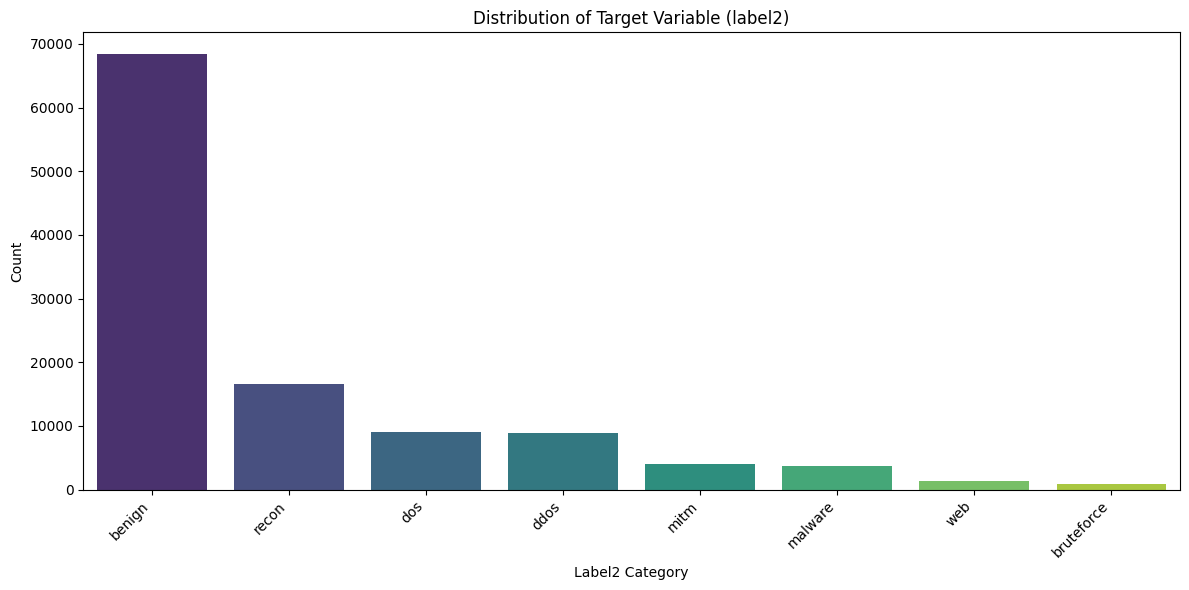
\includegraphics[width=5in]{Images/class_distribution.png}}
			{\rule{5in}{3.5in} % Placeholder -- add file at Images/class_distribution.png
			\\[-3.7in]\centering\textit{\small [Image not yet added: Images/class\_distribution.png]}\\[3.5in]}
	\end{center}
	\caption{Class distribution of the 8-category grouped label (benign plus seven attack categories) in the CIC IIoT 2025 evaluation subset: benign ($\approx$68{,}000), Recon ($\approx$16{,}500), DoS ($\approx$9{,}000), DDoS ($\approx$8{,}800), MITM ($\approx$4{,}000), Malware ($\approx$3{,}700), Web ($\approx$1{,}300), and Bruteforce ($<$1{,}000).}
	\label{fig:class_distribution}
\end{figure}

\textbf{Hardware and Software Environment:} The edge-layer models (GRU and Deep SVDD) were deployed on a simulated edge device using a [Insert Edge Hardware, e.g., Raspberry Pi 4 Model B with 4GB RAM]. As detailed in Section \ref{sec:edge_eval}, device-level latency and throughput benchmarking to date has been performed on the standalone baseline models compared against the proposed ensemble, run in a notebook development environment rather than on constrained edge hardware itself; benchmarking the deployed fused GRU + Deep SVDD ensemble under the same conditions, and repeating both on the target edge hardware, remains an open item noted in Section \ref{sec:limitations_integration}. The cloud-layer components run as a single Python process (a FastAPI application driven by \texttt{asyncio}, with no separate message broker or worker processes): a pre-trained XGBoost classifier and SHAP \texttt{TreeExplainer} for classification and explainability, and a LangChain-based Decision/Escalation Agent pipeline grounded by a FAISS vector store (falling back to a TF-IDF retriever when no embedding API key is configured) for the two LLM fallback touchpoints described in Section \ref{sec:multi_agent}. Because both the classifier and its explainer are tree-based rather than deep-learning models, this cloud tier has no GPU dependency; it was run on commodity CPU-only compute. The language-model calls in the \texttt{openai} configuration used [Insert Model, e.g., \texttt{gpt-4o-mini}] as the underlying LLM.

\textbf{Verification methodology:} In addition to the offline, dataset-driven evaluation of the edge-layer ensemble reported in Section \ref{sec:edge_eval}, the cloud-layer pipeline was verified through two rounds of live testing driven entirely over its two edge-facing HTTP endpoints, i.e. with a test harness playing the role of ``an edge layer,'' independently of this project's own edge-layer implementation (Section \ref{sec:limitations_integration} discusses why this separation was necessary). The first round exercised classification in isolation against a set of hand-crafted, unambiguous attack windows. The second round first performed a systematic grid search of the classifier's confidence boundary across roughly 40 traffic patterns at multiple volumes, then drove the full downstream chain-ladder escalation, edge apply/verification feedback, the final-tier approval gate, benign-state decay scheduling, both LLM fallback triggers, and the RAG self-learning write-back-end to end over HTTP for five representative scenarios. The findings from both rounds are reported in Sections \ref{sec:cloud_eval} and \ref{sec:mas_eval}.

\section{Edge Layer: Anomaly Detection Performance}\label{sec:edge_eval}

The proposed Cascaded Hybrid Ensemble (GRU + Deep SVDD) was benchmarked against eight alternative models trained and evaluated on the same held-out data: four standard supervised tree ensembles (Hist Gradient Boosting, Random Forest, Extra Trees, and the unsupervised Isolation Forest baseline), three classical linear/kernel classifiers (Gaussian Naive Bayes, Logistic Regression, and a Support Vector Classifier), and a standalone Deep SVDD model receiving only the point features, without the GRU's temporal embedding. This last comparison is the ensemble's ablation: it isolates what the GRU's temporal context specifically contributes, holding the Deep SVDD boundary itself fixed.

Table \ref{tb:edge_results} summarizes the detection performance of all nine models. The proposed ensemble achieved the highest score on every reported metric, and by a wide margin over standalone Deep SVDD specifically: accuracy improved by approximately 44.0 percentage points (55.6\% $\to$ 99.61\%), precision by approximately 46.4 points (53.3\% $\to$ 99.65\%), recall by approximately 8.8 points (91.0\% $\to$ 99.77\%), F1 by approximately 32.5 points (67.2\% $\to$ 99.71\%), and ROC-AUC by approximately 54.1 points (45.9\% $\to$ 99.98\%). Because the ensemble and the standalone Deep SVDD figures were produced by separate evaluation pipelines rather than a single controlled ablation run holding every other variable fixed, these deltas are reported here as descriptive rather than as a strictly paired ablation result, consistent with how the underlying evaluation itself qualifies the comparison. The direction and scale of the improvement are nonetheless consistent with the design argument of Section \ref{sec:hybrid_ensemble}: the GRU's temporal embedding gives Deep SVDD a materially richer representation to draw a boundary around than point features alone, particularly for recall, where standalone Deep SVDD's 91.0\% already indicates it detects most attacks in isolation but at the cost of far more false positives (53.3\% precision) than the fused ensemble ever exhibits. Figure \ref{fig:f1_benchmark} presents this same comparison visually, ranking all nine models by F1-score and showing the full five-metric heatmap side by side, which makes the size of the proposed ensemble's margin over every baseline immediately apparent.

\begin{table}[htbp]
\caption{Performance comparison of the proposed GRU + Deep SVDD ensemble against eight baseline models on the same held-out evaluation data.}
\label{tb:edge_results}
\begin{center}
\begin{tabular}{|l|c|c|c|c|}
\hline
\textbf{Model} & \textbf{Accuracy} & \textbf{Precision} & \textbf{Recall} & \textbf{F1-Score} \\
\hline
\textbf{GRU + Deep SVDD Ensemble} & \textbf{0.9961} & \textbf{0.9965} & \textbf{0.9977} & \textbf{0.9971} \\
\hline
Hist Gradient Boosting & 0.964 & 0.991 & 0.937 & 0.963 \\
\hline
Random Forest & 0.961 & 0.988 & 0.932 & 0.959 \\
\hline
Extra Trees & 0.958 & 0.990 & 0.925 & 0.957 \\
\hline
Isolation Forest & 0.886 & 0.904 & 0.864 & 0.883 \\
\hline
Gaussian Naive Bayes & 0.888 & 0.933 & 0.835 & 0.881 \\
\hline
Logistic Regression & 0.891 & 0.969 & 0.807 & 0.881 \\
\hline
Support Vector Classifier & 0.887 & 0.942 & 0.824 & 0.879 \\
\hline
Standalone Deep SVDD & 0.556 & 0.533 & 0.910 & 0.672 \\
\hline
\end{tabular}
\end{center}
\raggedright \textit{*Note: Standalone Deep SVDD receives point features only (no GRU temporal embedding) and constitutes the ablation baseline for the proposed ensemble.}
\end{table}

\begin{figure}[htbp]
	\begin{center}
		\IfFileExists{Images/edge/Fused GRU + Deep SVDD Against Individual Approaches.png}
			{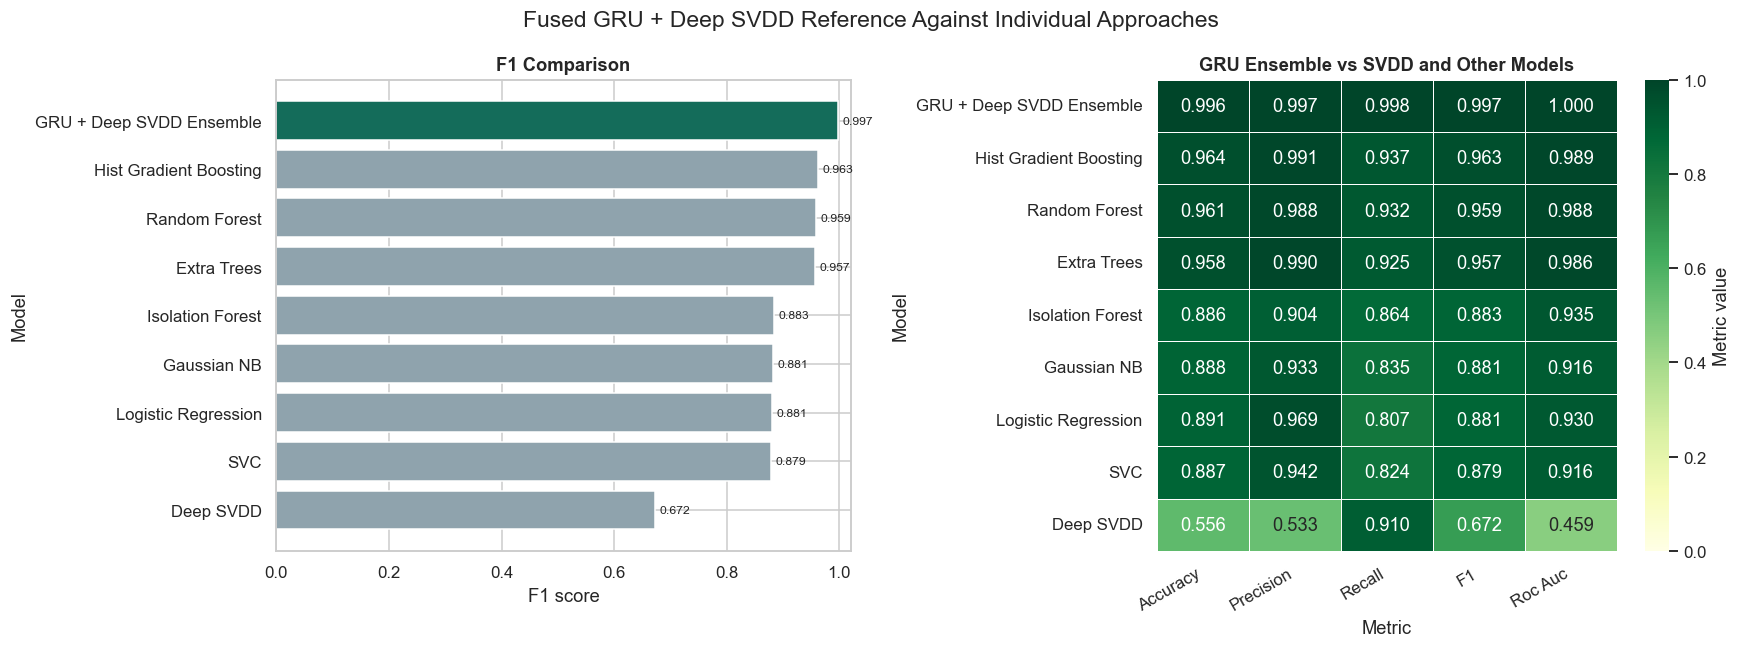
\includegraphics[width=5.5in]{Images/edge/Fused GRU + Deep SVDD Against Individual Approaches.png}}
			{\rule{5.5in}{4cm} % Placeholder -- add file at Images/edge/Fused GRU + Deep SVDD Against Individual Approaches.png
			\\[-4.2cm]\centering\textit{\small [Image not yet added: Images/f1\_benchmark\_comparison.png]}\\[4cm]}
	\end{center}
	\caption{F1-score comparison across all nine models (bar chart), alongside a heatmap of all five metrics per model, corresponding to the figures reported in Table \ref{tb:edge_results}.}
	\label{fig:f1_benchmark}
\end{figure}

Figure \ref{fig:fusion_comparison} isolates this ablation on its own axes, plotting the standalone Deep SVDD baseline against the fused ensemble across all five metrics so that the per-metric size of the fusion benefit-smallest for recall, largest for ROC-AUC-can be read directly rather than reconstructed from the percentage-point deltas above.

\begin{figure}[htbp]
	\begin{center}
		\IfFileExists{Images/edge/What fusion adds over standalone Deep SVDD.png}
			{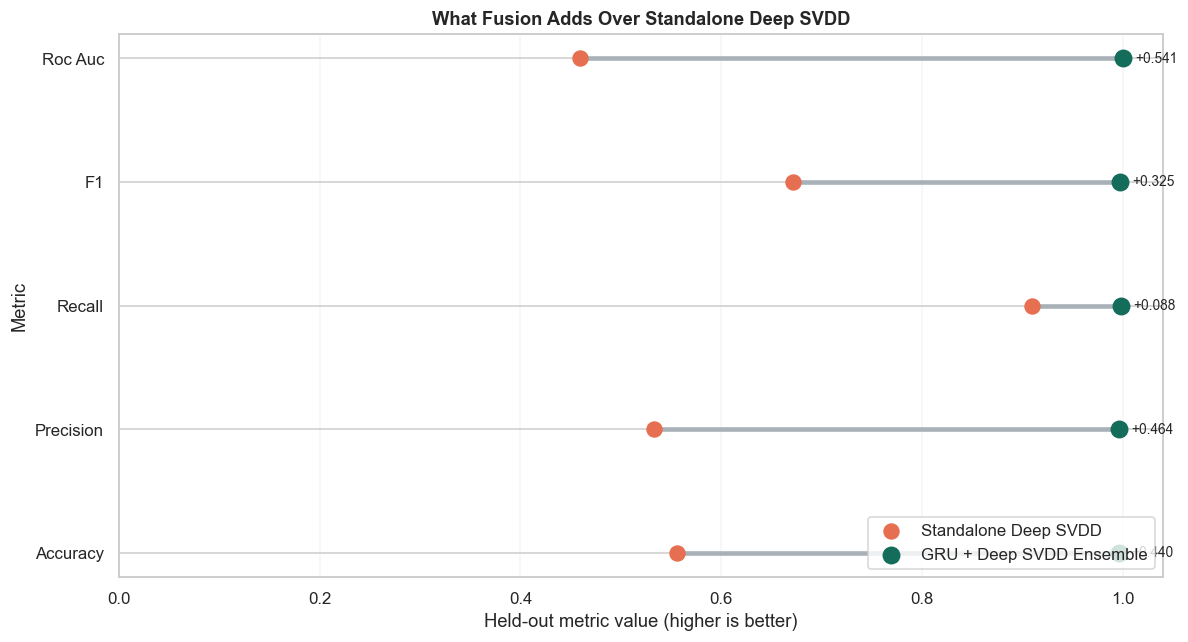
\includegraphics[width=5.5in]{Images/edge/What fusion adds over standalone Deep SVDD.png}}
			{\rule{5.5in}{4cm} % Placeholder -- add file at Images/edge/What fusion adds over standalone Deep SVDD.png
			\\[-4.2cm]\centering\textit{\small [Image not yet added: Images/fusion\_comparison.png]}\\[4cm]}
	\end{center}
	\caption{What fusion adds over standalone Deep SVDD: a per-metric comparison (accuracy, precision, recall, F1, ROC-AUC) between the standalone Deep SVDD baseline and the fused GRU + Deep SVDD ensemble, corresponding to the deltas discussed above.}
	\label{fig:fusion_comparison}
\end{figure}

At its selected operating threshold, the proposed ensemble's detailed classification breakdown on the 9{,}000-sample held-out set (3{,}000 benign, 6{,}000 attack) is reported in Table \ref{tb:edge_confusion} and visualised as a confusion matrix in Figure \ref{fig:confusion_matrix}. Of 3{,}000 benign windows, 21 were incorrectly flagged as attacks (a 0.70\% false-positive rate); of 6{,}000 attack windows, 14 were missed (a 0.23\% false-negative rate).

\begin{table}[htbp]
\caption{Confusion matrix and per-class detection metrics for the proposed GRU + Deep SVDD ensemble at its selected operating threshold.}
\label{tb:edge_confusion}
\centering
\begin{tabular*}{\textwidth}{@{\extracolsep{\fill}}|l|c|c|c|c|}
\hline
\textbf{Class} & \textbf{Precision} & \textbf{Recall} & \textbf{F1-Score} & \textbf{Support} \\
\hline
Normal (benign) & 0.9953 & 0.9930 & 0.9942 & 3{,}000 \\
\hline
Attack & 0.9965 & 0.9977 & 0.9971 & 6{,}000 \\
\hline
\end{tabular*}
\end{table}

\begin{figure}[htbp]
	\begin{center}
		\IfFileExists{Images/edge/Confusion Matrix GRU-SVDD.png}
			{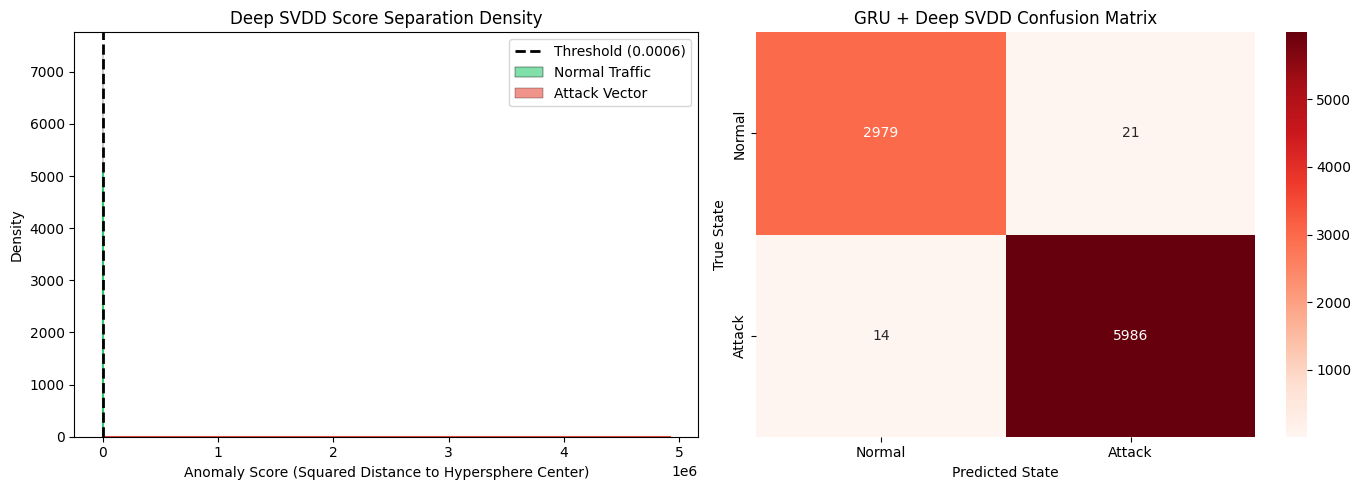
\includegraphics[width=5.5in]{Images/edge/Confusion Matrix GRU-SVDD.png}}
			{\rule{3.5in}{3.5in} % Placeholder -- add file at Images/edge/Confusion Matrix GRU-SVDD.png
			\\[-3.7in]\centering\textit{\small [Image not yet added: Images/confusion\_matrix.png]}\\[3.5in]}
	\end{center}
	\caption{Confusion matrix for the fused GRU + Deep SVDD ensemble at its selected operating threshold, corresponding to the figures reported in Table \ref{tb:edge_confusion}.}
	\label{fig:confusion_matrix}
\end{figure}

The operating threshold itself was selected via the same offline precision-recall/F1 search described in Section \ref{sec:hybrid_ensemble}, applied to the log-normalized distance score $d(v)$; the resulting threshold ($d(v) \approx 0.0006$) sits at the point where the precision and recall curves cross, balancing the two error types rather than minimising either in isolation. Figure \ref{fig:threshold_selection} shows the full basis for this choice: the log-normalized separation between benign and attack scores, the precision/recall/F1 trade-off curve, and the resulting false-positive/false-negative rate trade-off, with the selected threshold marked on each panel.

\begin{figure}[htbp]
	\begin{center}
		\IfFileExists{Images/edge/GRU + Deep SVDD Fused Anomaly_Benign Threshold Selection.png}
			{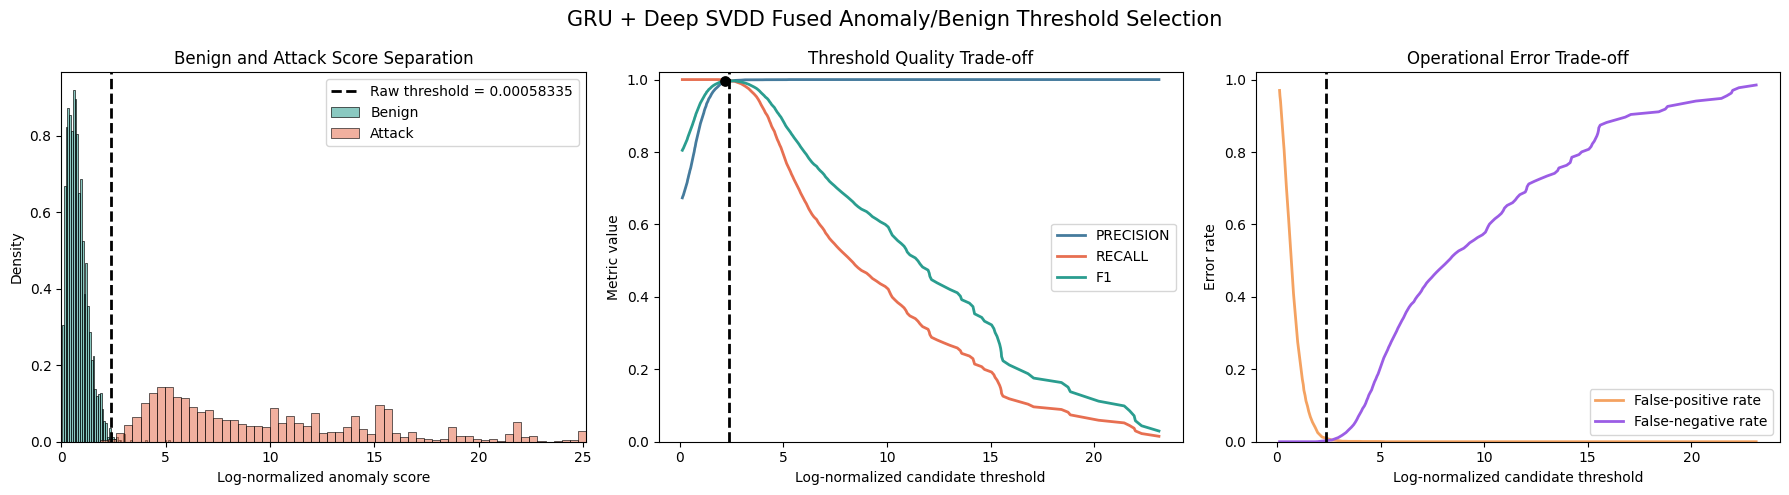
\includegraphics[width=\textwidth]{Images/edge/GRU + Deep SVDD Fused Anomaly_Benign Threshold Selection.png}}
			{\rule{5.5in}{4cm} % Placeholder -- add file at Images/edge/GRU + Deep SVDD Fused Anomaly_Benign Threshold Selection.png
			\\[-4.2cm]\centering\textit{\small [Image not yet added: Images/threshold\_selection.png]}\\[4cm]}
	\end{center}
	\caption{Threshold selection for the fused GRU + Deep SVDD score: benign/attack score separation on a log-normalized scale, the precision/recall/F1 trade-off curve, and the resulting false-positive/false-negative rate trade-off, with the selected operating threshold marked.}
	\label{fig:threshold_selection}
\end{figure}

\textbf{Edge-device hardware constraints.} Predictive quality must ultimately be balanced against the resource budget available on the target edge hardware (Chapter \ref{cha:introduction}). This trade-off was first characterised only for the baseline models evaluated in a notebook development environment: under those notebook conditions, the selected Random Forest configuration (250 trees, maximum depth 18) required 0.57 seconds to fit and scored the held-out batch in 0.0258 seconds, corresponding to approximately 309{,}543 rows per second; Hist Gradient Boosting scored the same batch in 0.0081 seconds (approximately 987{,}822 rows per second); and standalone Deep SVDD scored it in 0.0070 seconds (approximately 1{,}144{,}247 rows per second). These notebook-environment figures cover only the standalone baseline models and say nothing about the fused ensemble's own recurrent-inference and sequence-buffering overhead, nor about behaviour on the constrained target hardware itself, since large tree ensembles such as Random Forest additionally carry a memory and storage cost that a resource-constrained gateway may not be able to absorb regardless of raw throughput.

\textbf{On-device benchmark of the deployed fused ensemble.} The deployed, production GRU--Deep SVDD pipeline (artifact \texttt{gru-svdd-e3d39953d09f}) was subsequently benchmarked directly on a Raspberry Pi-class edge device (4-core ARM Cortex-A76, up to 2.4\,GHz, 8\,GiB RAM), closing part of the open item raised above. For each candidate CPU-thread configuration, 1{,}000 inferences were measured following 50 discarded warm-up runs; Table \ref{tb:edge_hw_benchmark} reports the resulting latency distribution and throughput.

\begin{table}[htbp]
\caption{On-device inference benchmark for the deployed fused GRU + Deep SVDD ensemble on the target Raspberry Pi-class gateway, across candidate CPU-thread configurations (1{,}000 measured inferences after 50 warm-up runs); all latency values are reported in milliseconds.}
\label{tb:edge_hw_benchmark}
\begin{center}
\begin{tabular}{|c|c|c|c|c|c|c|}
\hline
\textbf{Threads} & \textbf{Mean} & \textbf{Median} & \textbf{p95} & \textbf{p99} & \textbf{Max} & \textbf{Throughput (dec/s)} \\
\hline
\textbf{1} & \textbf{2.64} & \textbf{1.45} & \textbf{8.11} & \textbf{10.36} & 36.45 & \textbf{379} \\
\hline
2 & 2.78 & -- & -- & -- & -- & 360 \\
\hline
4 & 2.95 & 1.43 & 11.09 & 13.37 & 31.16 & 339 \\
\hline
\end{tabular}
\end{center}
\raggedright \textit{*Note: only the figures reported for the 1-thread and 4-thread configurations were directly available from the underlying benchmark run; the 2-thread row reports mean latency and throughput only.}
\end{table}

A single CPU thread gave the best balance of latency and throughput ($\approx$379 decisions/second at a mean latency of 2.64\,ms); two and four threads were both slower (360 and 339 decisions/second respectively), indicating that thread-management overhead outweighs any parallelism this comparatively compact model can exploit. Model initialisation took approximately 1.05 seconds with cached artifacts and approximately 4.28 seconds on a cold load, and the Python inference process reached a peak of approximately 332\,MiB RAM. Measured against the 2-second and 10-second scoring intervals the edge layer operates on (Chapter 3, Methodology), even the four-thread configuration's worst-case p99 latency (13.37\,ms) leaves substantial headroom, indicating that CPU and memory budget are not the binding constraint on scoring frequency for this ensemble on this hardware class.

Separately, the exported production model reports a detection quality of 0.913 F1, 99.49\% precision, 84.29\% recall, a ROC-AUC of 0.939, and a 1.97\% benign false-positive rate. These figures are noticeably weaker on recall than the 0.9971 F1 (99.65\% precision, 99.77\% recall) reported for the same ensemble on the notebook-evaluated held-out set in Table \ref{tb:edge_confusion}, and the gap is not yet reconciled: it may reflect a different train/evaluation split, a quantised or otherwise reduced export of the model used for the hardware benchmark, or a different operating threshold than the one selected in Figure \ref{fig:threshold_selection}. This discrepancy is noted here rather than resolved, consistent with this report's practice of surfacing rather than silently smoothing over inconsistencies between evaluation runs, and is carried forward as an open item in Section \ref{sec:limitations_integration}.

\section{Cloud Layer: Threat Classification and XAI}\label{sec:cloud_eval}

The cloud tier's classifier is trained against 76 fine-grained attack labels, grouped by summed class probability into the eight buckets described in Section \ref{sec:cloud_classification} (\texttt{benign}, \texttt{ddos}, \texttt{port\_scan}, \texttt{bruteforce}, \texttt{mirai\_botnet}, \texttt{lateral\_movement}, \texttt{exfiltration}, \texttt{unhandled\_attack}). Of the 30 numeric features the classifier expects, only a subset can be populated from data the edge layer actually forwards, because the edge sends connection-log-style aggregates rather than the packet-level captures (TCP window size, time-to-live statistics, maximum segment size, IP flags) the classifier was originally trained on; the remaining features are populated with a fixed placeholder value rather than left undefined. This is a structural mismatch between the granularity the model expects and the granularity the pipeline can supply, not a bug in either component individually, and it is the dominant factor behind the findings below.

\textbf{Offline validation on native features.} Before considering what happens when the edge layer supplies an incomplete feature vector, it is worth establishing whether the classification approach is sound at all when given the dataset's complete, native feature set. Table \ref{tb:offline_validation} reports validation performance for five candidate classifiers trained and evaluated at the 8-category grouped-label granularity (\texttt{label2}: benign plus the seven attack categories introduced in this chapter's Experimental Setup section above) on the same CIC IIoT 2025 subset. XGBoost was the strongest of the five, with 94.55\% accuracy and a macro F1-score of 92.60\%, ahead of Random Forest (93.09\%, 91.12\%), KNeighbors (92.83\%, 88.45\%), and Decision Tree (92.32\%, 89.49\%); GaussianNB was markedly weaker on every metric (76.47\% accuracy, 53.86\% macro F1), consistent with a linear-boundary model struggling against the non-linear decision boundaries a tree ensemble captures naturally. Figure \ref{fig:validation_accuracy} plots this same accuracy ranking, making GaussianNB's gap from the other four candidates visually unambiguous.

\begin{table}[htbp]
\caption{Offline validation performance of five candidate classifiers at the 8-category grouped-label granularity, evaluated on the CIC IIoT 2025 dataset with its complete native feature set.}
\label{tb:offline_validation}
\begin{center}
\begin{tabular}{|l|c|c|c|c|}
\hline
\textbf{Model} & \textbf{Accuracy} & \textbf{Macro Precision} & \textbf{Macro Recall} & \textbf{Macro F1-score} \\
\hline
\textbf{XGBoost} & \textbf{0.9455} & \textbf{0.9702} & 0.8887 & \textbf{0.9260} \\
\hline
Random Forest & 0.9309 & 0.9419 & 0.8842 & 0.9112 \\
\hline
KNeighbors & 0.9283 & 0.9337 & 0.8436 & 0.8845 \\
\hline
Decision Tree & 0.9232 & 0.9183 & 0.8735 & 0.8949 \\
\hline
GaussianNB & 0.7647 & 0.5947 & 0.5894 & 0.5386 \\
\hline
\end{tabular}
\end{center}
\end{table}

\begin{figure}[htbp]
	\begin{center}
		\IfFileExists{Images/validation_accuracy_comparison.png}
			{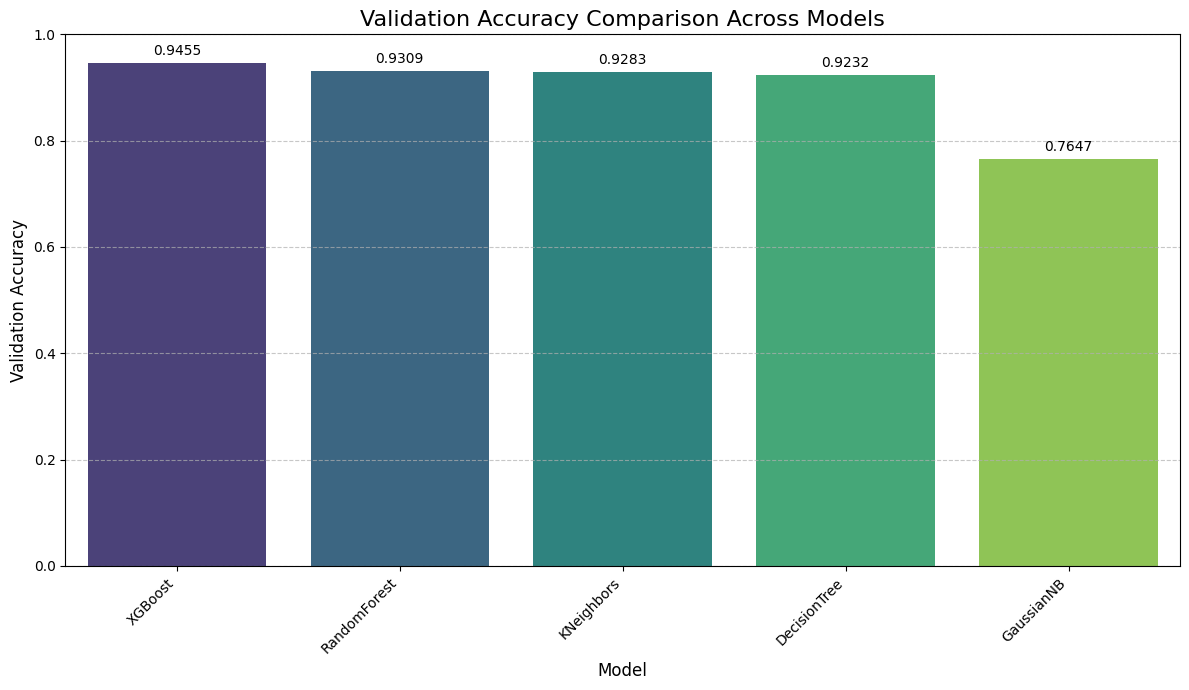
\includegraphics[width=5in]{Images/validation_accuracy_comparison.png}}
			{\rule{5in}{3.5in} % Placeholder -- add file at Images/validation_accuracy_comparison.png
			\\[-3.7in]\centering\textit{\small [Image not yet added: Images/validation\_accuracy\_comparison.png]}\\[3.5in]}
	\end{center}
	\caption{Validation accuracy comparison across the five candidate classifiers reported in Table \ref{tb:offline_validation}.}
	\label{fig:validation_accuracy}
\end{figure}

This result is a useful counterpoint to the live findings that follow: it indicates that XGBoost, given the features it was actually designed around, discriminates this dataset's attack categories well. The gap between this offline result and the live, edge-simulated findings below is consequently attributable to the feature-completeness gap described above, not to the underlying classification approach being unsound. XGBoost's macro recall (88.87\%) was nonetheless the weakest of its four reported metrics, and not uniformly so across classes: two of the eight categories showed recall as low as 77.86\% and 81.72\% respectively even with the complete native feature set, indicating that some attack categories are harder to separate from the majority-benign traffic than others regardless of feature completeness, a caveat worth carrying forward alongside the feature-gap explanation rather than treating the offline result as an unqualified upper bound.

The systematic confidence-boundary probe described in this chapter's Experimental Setup section above-roughly 40 traffic patterns evaluated against the live classifier across a range of record volumes per window-produced the following findings, each independently reproduced rather than observed once:

\begin{itemize}
	\item \textbf{False negatives at high confidence.} Port scans, SSH/Telnet dictionary brute-force attempts, and Mirai-style outbound scanning traffic were classified as \texttt{benign} at 90--98\% confidence across every volume tested (50 to 20,000 records per window)-never once crossing into a detected state.
	\item \textbf{False positives at high confidence.} A purely legitimate, heavy but ordinary HTTPS session was classified \texttt{ddos} at 55\% confidence. This was reproduced end to end through the full downstream pipeline, and it dispatched real containment actions (flood hardening and rate limiting, \texttt{NET-02} + \texttt{NET-01}) against a device that was never actually under attack.
	\item \textbf{Confidence is non-monotonic with attack volume.} A SYN flood crossed the confidence gate at 50 records per window; the same attack pattern at 300 records did not; at 1,000 or more records it flipped to a confidently \texttt{benign} classification. Confidence at this classifier's output is consequently not a reliable proxy for attack severity, or even attack presence, in this pipeline.
	\item \textbf{The fine-grained label is frequently wrong even when the grouped bucket's gate is crossed.} UDP floods were classified into fine-grained labels such as \texttt{unhandled\_attack} or \texttt{web\_sql-injection} rather than any \texttt{ddos}-family label, even in cases where a large-payload flood happened to land on a correct \texttt{ddos} fine label.
\end{itemize}

Taken together, these findings indicate that classification accuracy on real-world, connection-log-shaped input is the dominant limitation of the cloud tier as currently integrated, in both directions: attacks are missed, and benign traffic is acted against. This is discussed further, alongside its likely cause and possible remediations, in Section \ref{sec:limitations_integration}.

Crucially, the classification is still passed through a SHAP explainer regardless of its correctness, computed against the predicted fine-grained label. The top-3 contributing features by $|\phi_i|$ (Equation \ref{e:shap}) are translated into short plain-English statements-for example, describing a high count of unanswered SYN packets as evidence pushing the classification toward a particular attack class-and this translated attribution, rather than the raw SHAP vector, is what is passed to the Dashboard Reporting Agent and to either LLM fallback agent when one is consulted. The explainer's correctness is bounded by the classifier's own correctness: SHAP faithfully explains \textit{why} the model produced a given output, but on the evidence above it cannot compensate for the model being asked to classify against features it was never actually given.

\subsection{Explanation-Quality Metrics}\label{sec:xai_eval}

Because the healing pipeline consumes SHAP attributions as first-class evidence rather than as an advisory overlay, the attributions were evaluated as a subsystem in their own right, in addition to the correctness deletion curve reported in Section \ref{sec:cloud_classification} (Figure \ref{fig:correctness_deletion}, AUPC = 0.1264). The four metrics reported below assess complementary properties: completeness (do the attributions add up to what the model actually output?), continuity (do neighbouring inputs receive comparable explanations?), contrastivity (do different attack classes rely on distinguishably different feature sets?), compactness (how few features are needed to account for most of the attribution mass?), and global feature importance (which features drive one representative class overall?).

\textbf{Completeness (additivity).} SHAP's defining property is that the model's output for a given sample should equal the baseline prediction plus the sum of the per-feature contributions, so a residual close to zero indicates that the returned explanation faithfully reproduces the model output rather than approximating it. Figure \ref{fig:xai_completeness} plots the distribution of absolute residuals $|f(x) - (\text{base value} + \sum_i \phi_i)|$ across the evaluation set. The values are concentrated at an extremely small scale (on the order of $10^{-6}$), with virtually the entire distribution below $5 \times 10^{-6}$, which is strong evidence that the SHAP implementation used here is numerically complete and that the summed contributions reconstruct the raw model output with negligible error.

\begin{figure}[htbp]
	\begin{center}
		\IfFileExists{Images/xai_evaluation/completeness_residuals.jpeg}
			{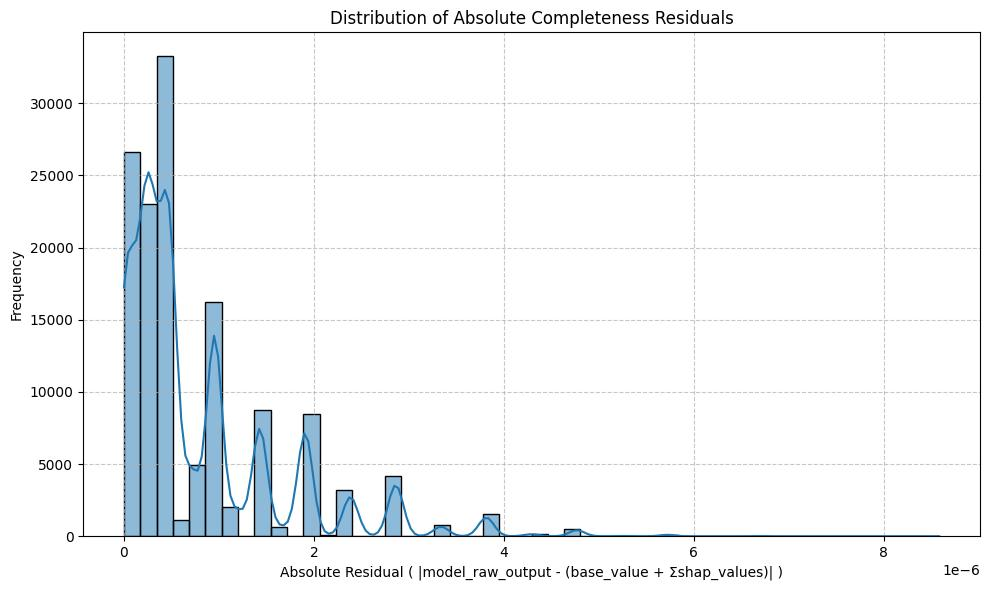
\includegraphics[width=5.5in]{Images/xai_evaluation/completeness_residuals.jpeg}}
			{\rule{5.5in}{3in}
			\\[-3.2cm]\centering\textit{\small [Image not yet added: Images/xai\_evaluation/completeness\_residuals.jpeg]}\\[3in]}
	\end{center}
	\caption{Distribution of absolute completeness residuals, $|f(x) - (\text{base value} + \sum_i \phi_i)|$, across the evaluation set. The residuals are concentrated at the $10^{-6}$ scale, confirming that the SHAP attributions returned by the pipeline reconstruct the raw model output to within numerical noise.}
	\label{fig:xai_completeness}
\end{figure}

\textbf{Continuity (explanation stability).} Continuity measures the average absolute change in SHAP values between comparable or neighbouring samples, capturing whether small input variations produce correspondingly small attribution changes rather than arbitrary shifts. The average continuity score on this classifier is 0.7787 (Figure \ref{fig:xai_continuity}), with the histogram showing that per-sample explanation changes span a range rather than being uniformly near zero. This indicates moderate-to-good continuity: attributions are stable in bulk, but not perfectly so, and some neighbouring windows do receive noticeably different attributions. This is expected near classifier decision boundaries and in regions where network-traffic behaviour changes abruptly between windows, and it is consistent with the non-monotonic-confidence finding reported earlier in this section: where the classifier's own output shifts sharply with small input changes, its explanations shift with it.

\begin{figure}[htbp]
	\begin{center}
		\IfFileExists{Images/xai_evaluation/continuity_distribution.jpeg}
			{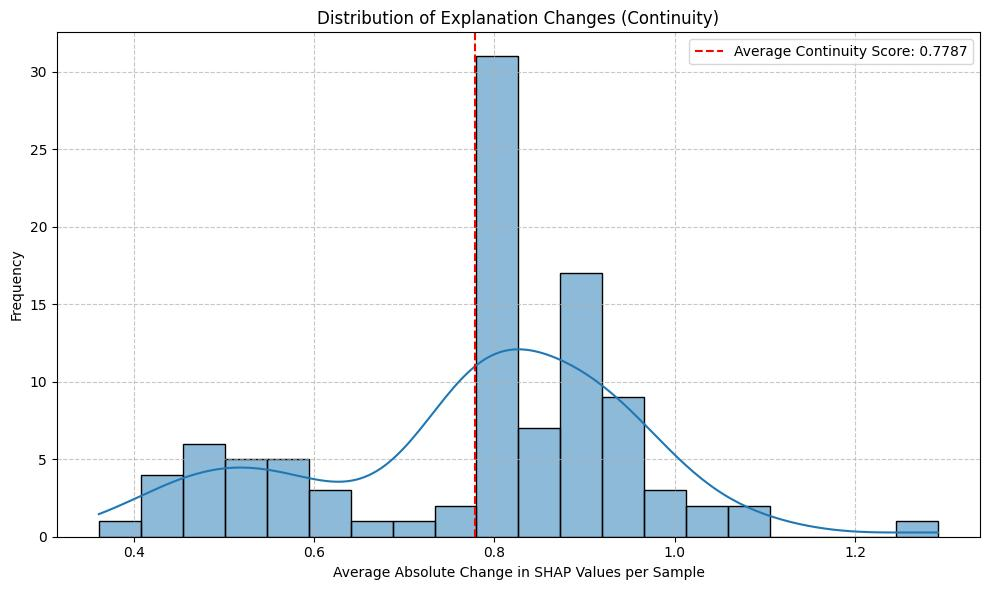
\includegraphics[width=5.5in]{Images/xai_evaluation/continuity_distribution.jpeg}}
			{\rule{5.5in}{3in}
			\\[-3.2cm]\centering\textit{\small [Image not yet added: Images/xai\_evaluation/continuity\_distribution.jpeg]}\\[3in]}
	\end{center}
	\caption{Distribution of per-sample explanation changes (continuity). The dashed line marks the average continuity score of 0.7787; the spread indicates moderate-to-good stability, with the tail representing samples near classifier decision boundaries where attributions shift more sharply.}
	\label{fig:xai_continuity}
\end{figure}

\textbf{Contrastivity (class discrimination).} Contrastivity measures the Jaccard distance between the sets of top-10 influential features for each pair of predicted classes: a value of 0.00 means both classes rely on identical top-10 feature sets, while 1.00 means the two classes share no top-10 features at all, so larger values indicate more class-specific explanations. Figure \ref{fig:xai_contrastivity} shows the resulting pairwise heatmap over the eight grouped labels. Most off-diagonal values sit between 0.46 and 0.75, so the classifier's explanations are largely contrastive across attack families. The one notable exception is the \texttt{ddos}--\texttt{recon} pair at 0.18, which indicates substantial overlap in top-attributed features between DDoS and reconnaissance windows-plausible given that both classes are dominated by network-volume and packet-pattern indicators, and worth targeted feature-overlap and confusion analysis. The highest observed distances (0.75) occur for multiple pairs, including \texttt{benign}--\texttt{bruteforce}, \texttt{benign}--\texttt{dos}, \texttt{benign}--\texttt{web}, \texttt{dos}--\texttt{mitm}, \texttt{malware}--\texttt{mitm}, and \texttt{mitm}--\texttt{web}, indicating that these class pairs are being explained through effectively disjoint feature sets.

\begin{figure}[htbp]
	\begin{center}
		\IfFileExists{Images/xai_evaluation/contrastivity_jaccard.jpeg}
			{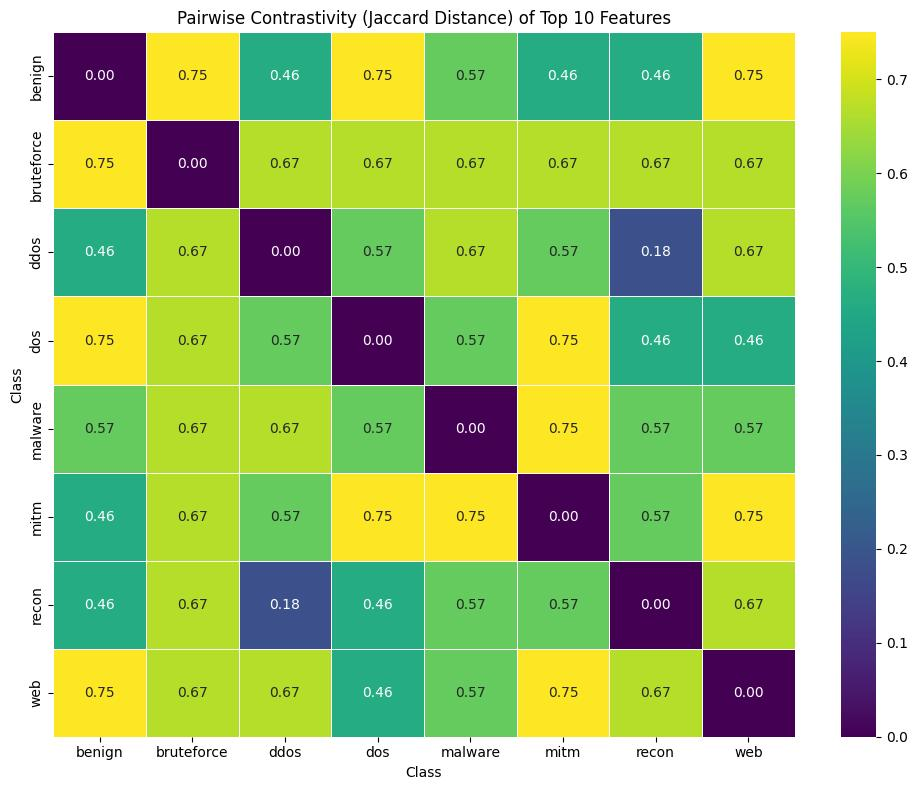
\includegraphics[width=5in]{Images/xai_evaluation/contrastivity_jaccard.jpeg}}
			{\rule{5in}{4in}
			\\[-4.2cm]\centering\textit{\small [Image not yet added: Images/xai\_evaluation/contrastivity\_jaccard.jpeg]}\\[4in]}
	\end{center}
	\caption{Pairwise contrastivity (Jaccard distance) between the top-10 influential features of each pair of predicted classes. Higher values indicate more class-specific explanations; the \texttt{ddos}--\texttt{recon} entry at 0.18 is the main low-contrastivity outlier and is flagged for targeted feature-overlap analysis.}
	\label{fig:xai_contrastivity}
\end{figure}

\textbf{Compactness.} For each sample, the number of features $k$ needed to account for 90\% of the total absolute attribution mass was computed after sorting features by $|\phi_i|$. The average across the evaluation set is $k \approx 9.13$: although the classifier consumes a 30-feature vector, roughly nine features usually explain the bulk of any given prediction. This is directly useful for the downstream healing pipeline, since the top-3 statements passed to the Dashboard Reporting Agent and the LLM fallback agents (Section \ref{sec:multi_agent}) are drawn from precisely this concentrated head of the attribution ranking rather than from a diffuse feature cloud.

\textbf{Global feature importance for the benign class.} Figure \ref{fig:xai_shap_benign} reports the mean absolute SHAP value per feature for the \texttt{benign} output across the evaluation set, expressing global importance magnitude but not direction. The leading features are \path{network_packet-size_min}, \path{network_packets_all_count}, \path{network_window-size_min}, \path{network_ip-length_min}, and \path{network_window-size_max}, followed by \path{network_ports_dst_count}, \path{network_ips_all_count}, and \path{log_data-types}. The \texttt{benign} decision is therefore shaped predominantly by packet-size, packet-count, TCP-window, and IP-length behaviour, which is plausible for traffic classification given that benign traffic typically has a characteristic distribution of flow sizes, packet volumes, and protocol-level properties. Two caveats apply. First, global importance does not establish causality, and the bar chart does not indicate whether a high or low value of each feature increases or decreases the probability of the \texttt{benign} class; per-sample directional plots are the appropriate instrument for that question. Second, this ranking must be read against the granularity mismatch flagged earlier in this section: several of the leading features are precisely the packet-level signals the current edge layer does not natively forward, so the very features on which the model relies most for a \texttt{benign} verdict are the ones most exposed to placeholder-value inference at runtime.

\begin{figure}[htbp]
	\begin{center}
		\IfFileExists{Images/xai_evaluation/shap_importance_benign.jpeg}
			{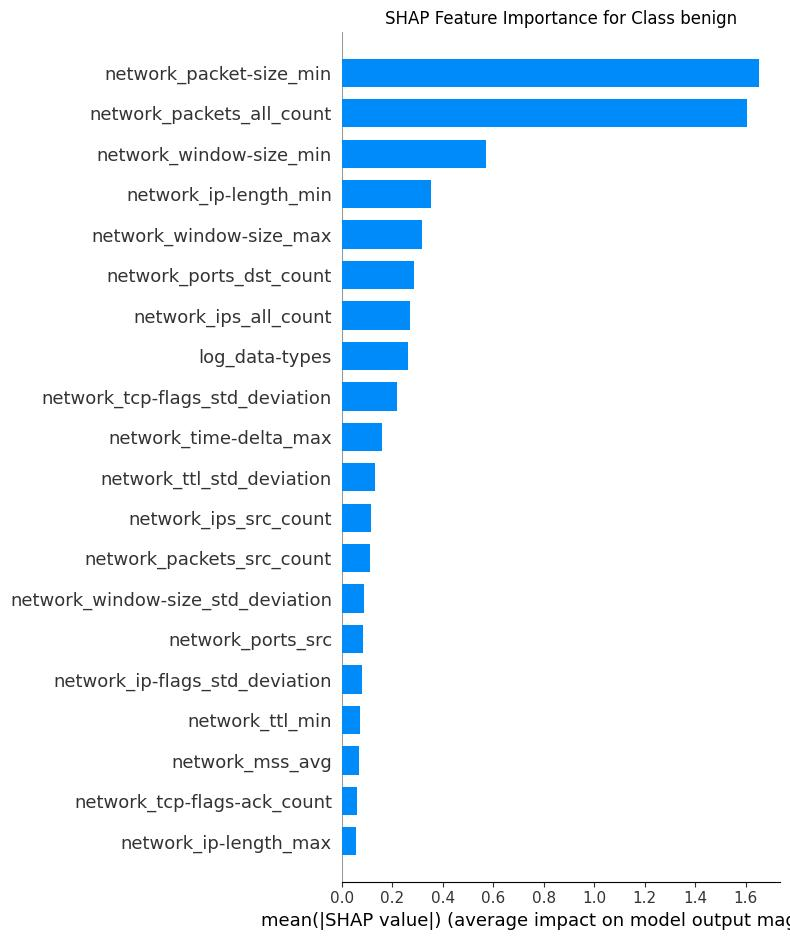
\includegraphics[width=5in]{Images/xai_evaluation/shap_importance_benign.jpeg}}
			{\rule{5in}{4in}
			\\[-4.2cm]\centering\textit{\small [Image not yet added: Images/xai\_evaluation/shap\_importance\_benign.jpeg]}\\[4in]}
	\end{center}
	\caption{Mean absolute SHAP value per feature for the \texttt{benign} class across the evaluation set. Packet-size, packet-count, TCP-window, and IP-length features dominate the \texttt{benign} decision; several of these are also the packet-level signals most affected by the edge-side granularity mismatch discussed in this section.}
	\label{fig:xai_shap_benign}
\end{figure}

\textbf{Per-class global importance across the seven attack families.} The same mean-$|\phi_i|$ ranking was computed for each of the seven attack-class outputs; the results are shown as a grid in Figure \ref{fig:xai_importance_attacks}. Four of the seven classes-\texttt{ddos}, \texttt{dos}, \texttt{malware}, and \texttt{recon}-are led by \path{network_packets_all_count}, indicating that the classifier's top signal for all four is total-volume-per-window rather than any structural fingerprint distinguishing them from one another. This is the same overlap flagged by the contrastivity heatmap (Figure \ref{fig:xai_contrastivity}), where the smallest non-diagonal Jaccard distance was recorded between \texttt{ddos} and \texttt{recon} at 0.18, and it is the most likely explanatory cause of the fine-grained-label errors reported earlier in this section (UDP floods landing on \texttt{unhandled\_attack} or \texttt{web\_sql-injection} rather than a \texttt{ddos}-family label). The remaining three classes are distinguished by different leading features: \texttt{bruteforce} is led by \path{network_time-delta_max}, consistent with the paced, retry-driven timing signature of dictionary attacks; \texttt{mitm} by \path{network_packet-size_min}, consistent with the small, manipulated packets characteristic of man-in-the-middle interception; and \texttt{web} by \path{network_ttl_max}, consistent with the extra routing hops incurred by many web-application attack paths. Log-level features (for example \path{log_data-types}) appear in the top-20 for most classes but rarely near the top, reflecting the classifier's overall bias toward network-layer signals over application-log signals on this feature schema.

\begin{figure}[htbp]
	\centering
	\begin{subfigure}[t]{0.48\textwidth}
		\centering
		\IfFileExists{Images/xai_evaluation/shap_importance_ddos.jpeg}
			{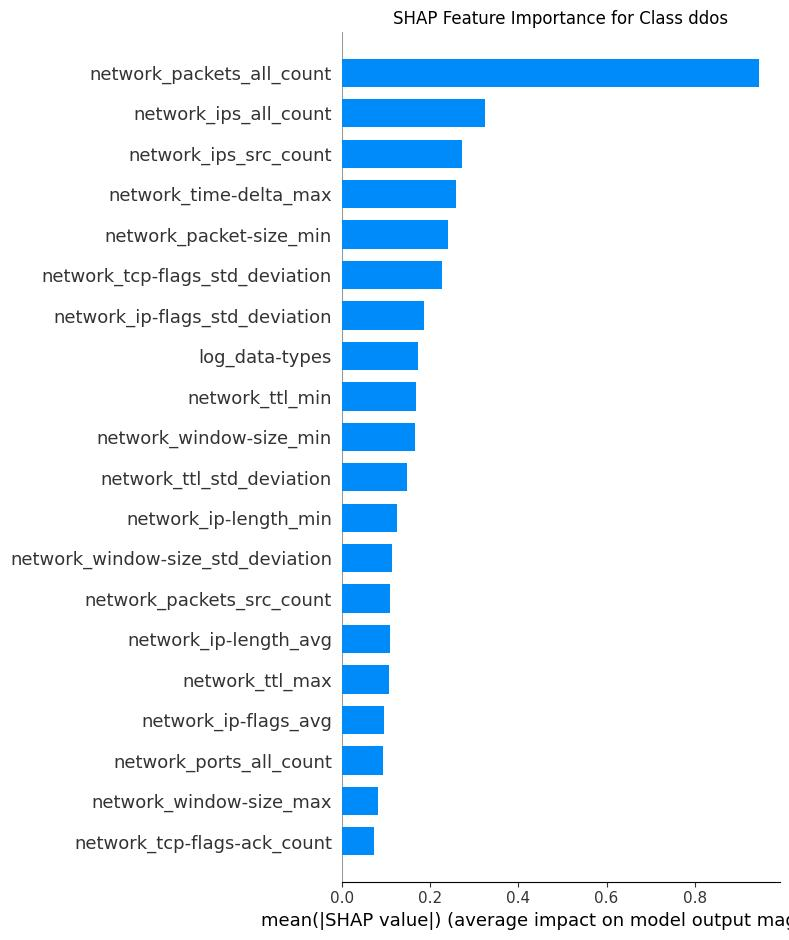
\includegraphics[width=\linewidth]{Images/xai_evaluation/shap_importance_ddos.jpeg}}
			{\rule{\linewidth}{2in}}
		\caption{\texttt{ddos}}
	\end{subfigure}
	\hfill
	\begin{subfigure}[t]{0.48\textwidth}
		\centering
		\IfFileExists{Images/xai_evaluation/shap_importance_dos.jpeg}
			{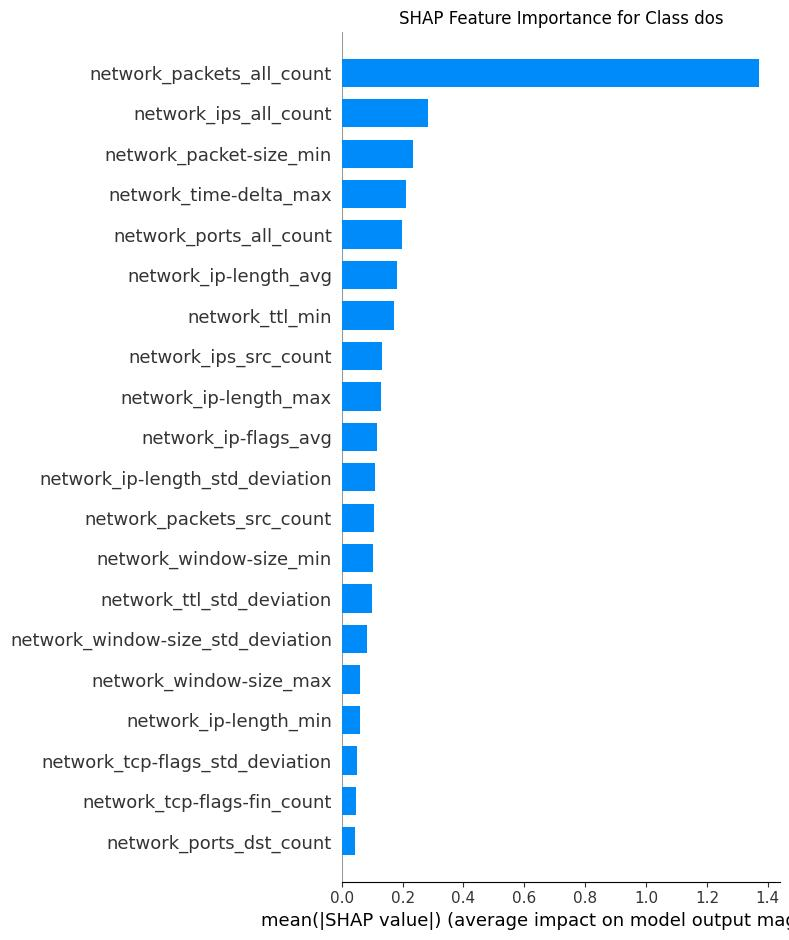
\includegraphics[width=\linewidth]{Images/xai_evaluation/shap_importance_dos.jpeg}}
			{\rule{\linewidth}{2in}}
		\caption{\texttt{dos}}
	\end{subfigure}

	\vspace{0.5em}

	\begin{subfigure}[t]{0.48\textwidth}
		\centering
		\IfFileExists{Images/xai_evaluation/shap_importance_recon.jpeg}
			{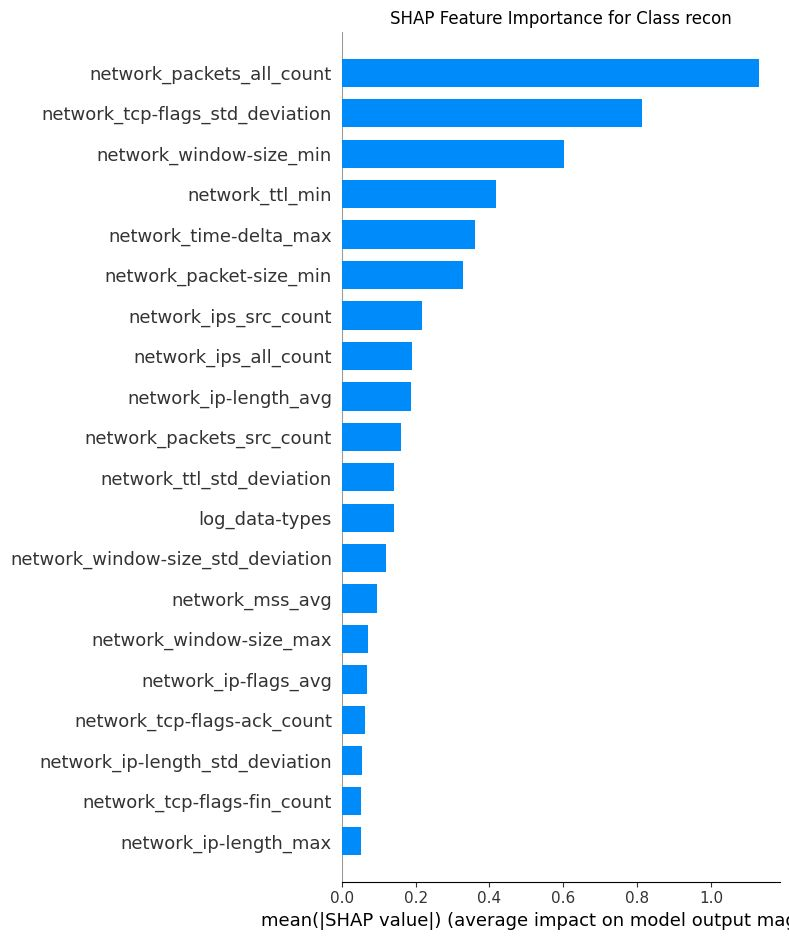
\includegraphics[width=\linewidth]{Images/xai_evaluation/shap_importance_recon.jpeg}}
			{\rule{\linewidth}{2in}}
		\caption{\texttt{recon}}
	\end{subfigure}
	\hfill
	\begin{subfigure}[t]{0.48\textwidth}
		\centering
		\IfFileExists{Images/xai_evaluation/shap_importance_malware.jpeg}
			{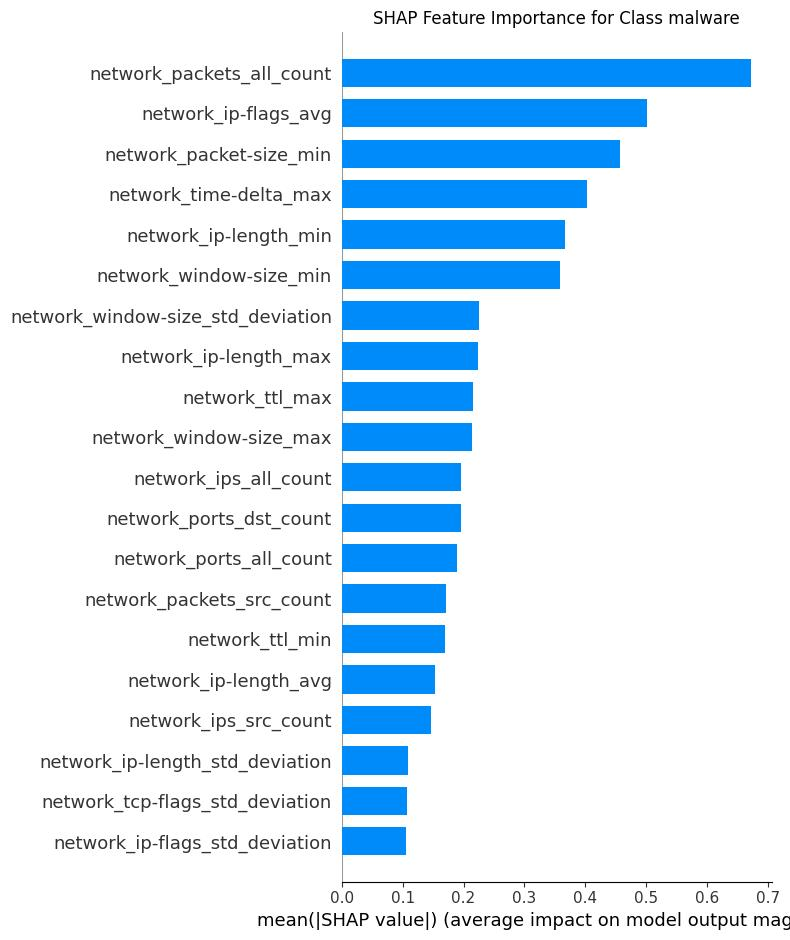
\includegraphics[width=\linewidth]{Images/xai_evaluation/shap_importance_malware.jpeg}}
			{\rule{\linewidth}{2in}}
		\caption{\texttt{malware}}
	\end{subfigure}
	\caption{Mean absolute SHAP value per feature (top-20) for the four volume-led attack-class outputs. All four are led by \texttt{network\_packets\_all\_count}, consistent with the low pairwise-contrastivity outlier flagged in Figure \ref{fig:xai_contrastivity}.}
	\label{fig:xai_importance_attacks}
\end{figure}

\begin{figure}[htbp]\ContinuedFloat
	\centering
	\begin{subfigure}[t]{0.32\textwidth}
		\centering
		\IfFileExists{Images/xai_evaluation/shap_importance_bruteforce.jpeg}
			{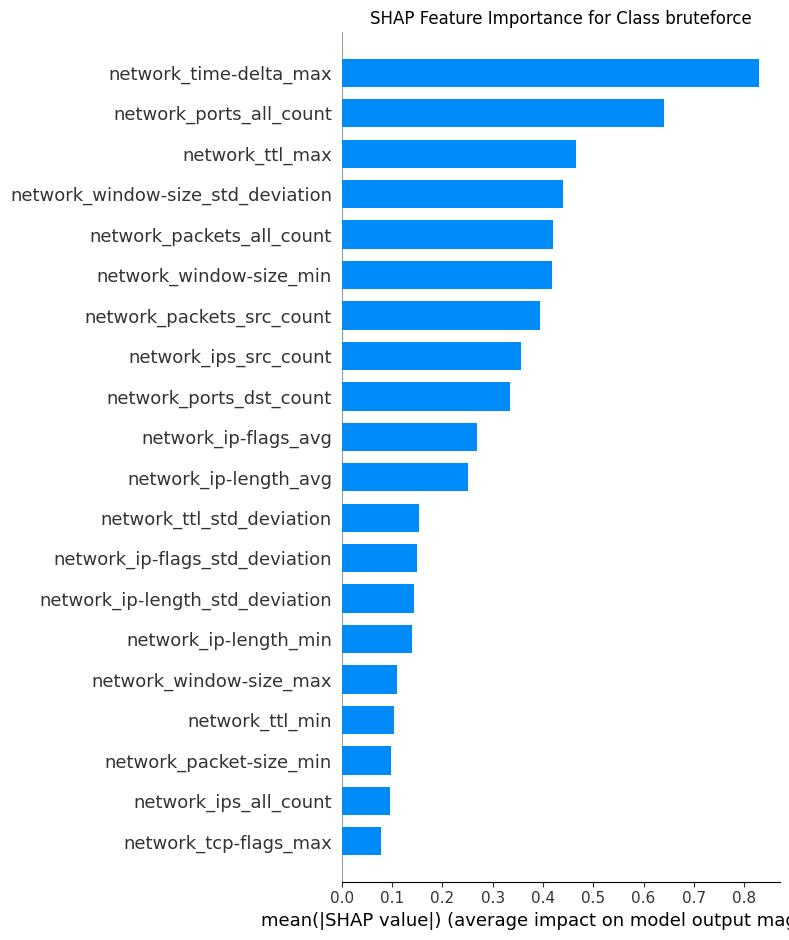
\includegraphics[width=\linewidth]{Images/xai_evaluation/shap_importance_bruteforce.jpeg}}
			{\rule{\linewidth}{2in}}
		\caption{\texttt{bruteforce}}
	\end{subfigure}
	\hfill
	\begin{subfigure}[t]{0.32\textwidth}
		\centering
		\IfFileExists{Images/xai_evaluation/shap_importance_mitm.jpeg}
			{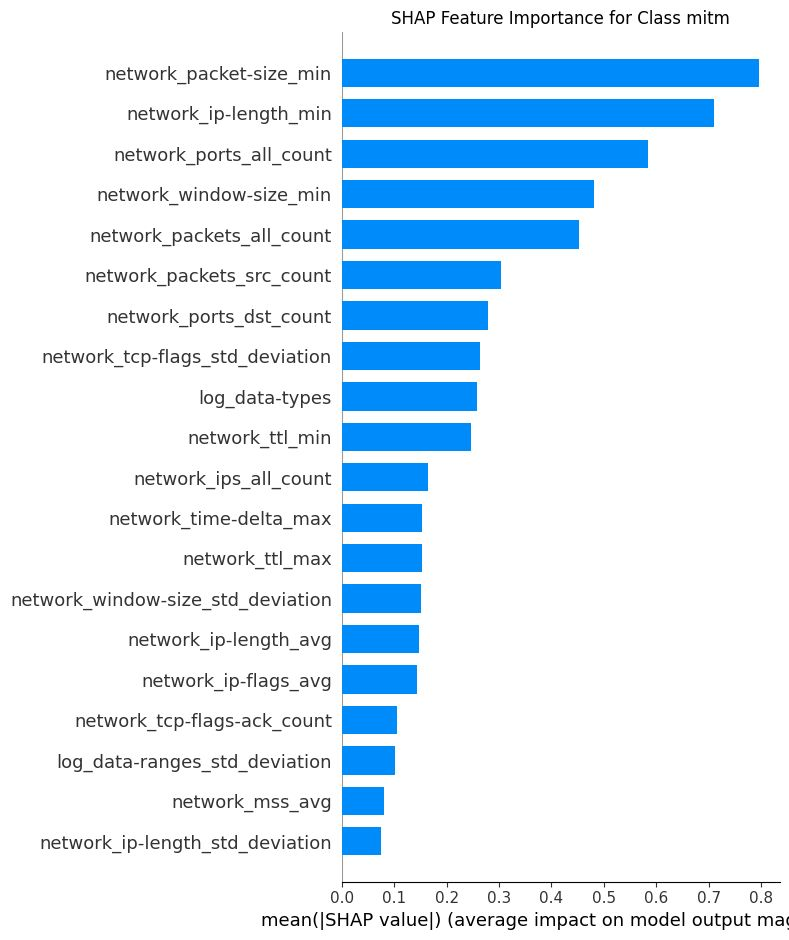
\includegraphics[width=\linewidth]{Images/xai_evaluation/shap_importance_mitm.jpeg}}
			{\rule{\linewidth}{2in}}
		\caption{\texttt{mitm}}
	\end{subfigure}
	\hfill
	\begin{subfigure}[t]{0.32\textwidth}
		\centering
		\IfFileExists{Images/xai_evaluation/shap_importance_web.jpeg}
			{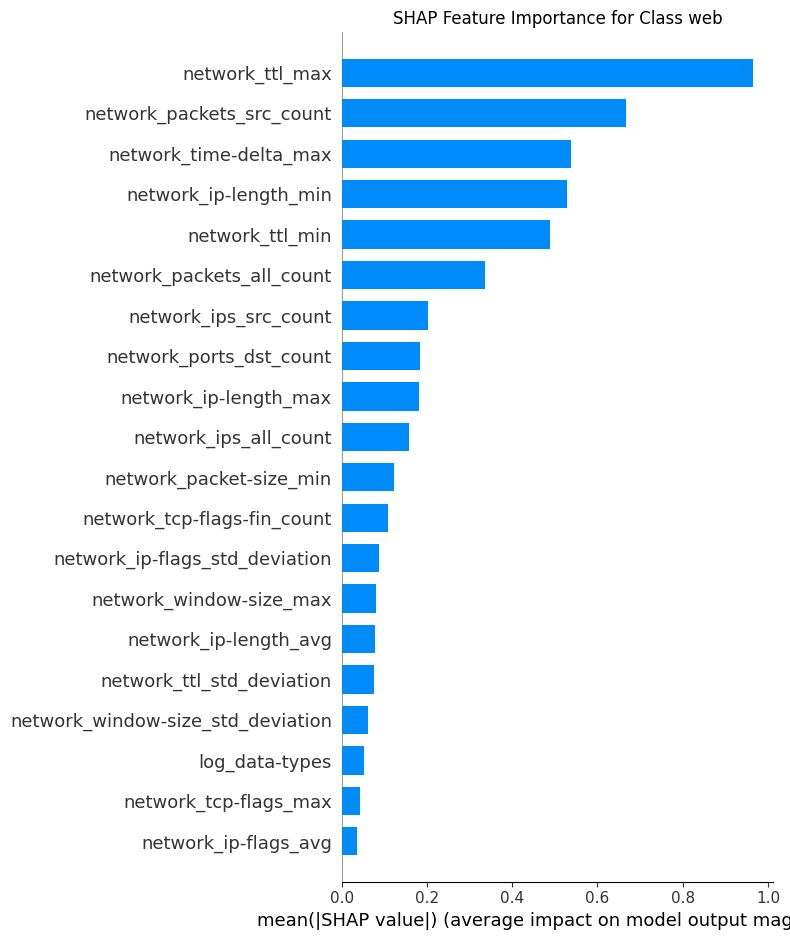
\includegraphics[width=\linewidth]{Images/xai_evaluation/shap_importance_web.jpeg}}
			{\rule{\linewidth}{2in}}
		\caption{\texttt{web}}
	\end{subfigure}
	\caption{Mean absolute SHAP value per feature (top-20) for the three distinct-signature attack-class outputs. \texttt{bruteforce}, \texttt{mitm}, and \texttt{web} are distinguished by timing, small-packet, and TTL-based leading features respectively.}
	\label{fig:xai_importance_attacks_distinct}
\end{figure}

\FloatBarrier

\textbf{Directional analysis via SHAP summary plots.} The bar-chart importance ranking captures magnitude but not the direction in which each feature pushes the class output, and does not reveal whether the relationship between feature value and SHAP contribution is monotonic or not. Figure \ref{fig:xai_summary_attacks} shows the corresponding SHAP summary (beeswarm) plots for the same seven classes: each point represents one sample-feature pair, its horizontal position is the SHAP value contributed by that feature for that sample, and its colour encodes the raw feature value from low (blue) to high (red). Positive SHAP values on the horizontal axis push the model toward the class in question and negative values push it away, so a feature whose high-value points cluster on the right supports the class when observed at a high value, and one whose high-value points cluster on the left opposes it. Two systematic patterns emerge across the attack classes. First, the beeswarms for the four volume-led classes (\texttt{ddos}, \texttt{dos}, \texttt{malware}, \texttt{recon}) show a long red tail of \path{network_packets_all_count} points on the positive side, confirming that high packet counts per window push the model toward each of these attack labels as expected, but also that the same directional signal is being reused for all four. Second, several features show pronounced non-linearity: for \texttt{mitm}, both very-low and moderate values of \path{network_packet-size_min} can produce large positive SHAP values, indicating that the model does not treat this feature as a simple threshold. The wide horizontal spreads visible on the top-ranked features across every class are also the direct empirical explanation for the moderate continuity score reported earlier (0.7787, Figure \ref{fig:xai_continuity}): where a single feature can contribute across a broad SHAP range depending on its raw value, small input differences will produce correspondingly wider attribution differences than they would for a strictly monotonic classifier.

\begin{figure}[htbp]
	\centering
	\begin{subfigure}[t]{0.48\textwidth}
		\centering
		\IfFileExists{Images/xai_evaluation/shap_summary_ddos.jpeg}
			{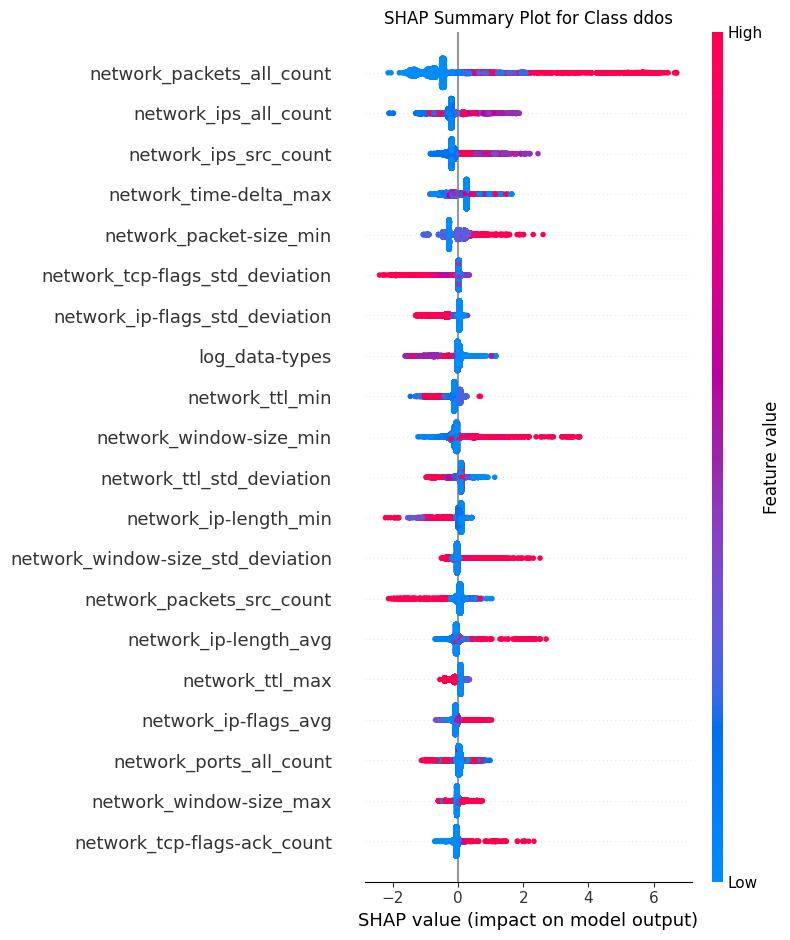
\includegraphics[width=\linewidth]{Images/xai_evaluation/shap_summary_ddos.jpeg}}
			{\rule{\linewidth}{2in}}
		\caption{\texttt{ddos}}
	\end{subfigure}
	\hfill
	\begin{subfigure}[t]{0.48\textwidth}
		\centering
		\IfFileExists{Images/xai_evaluation/shap_summary_dos.jpeg}
			{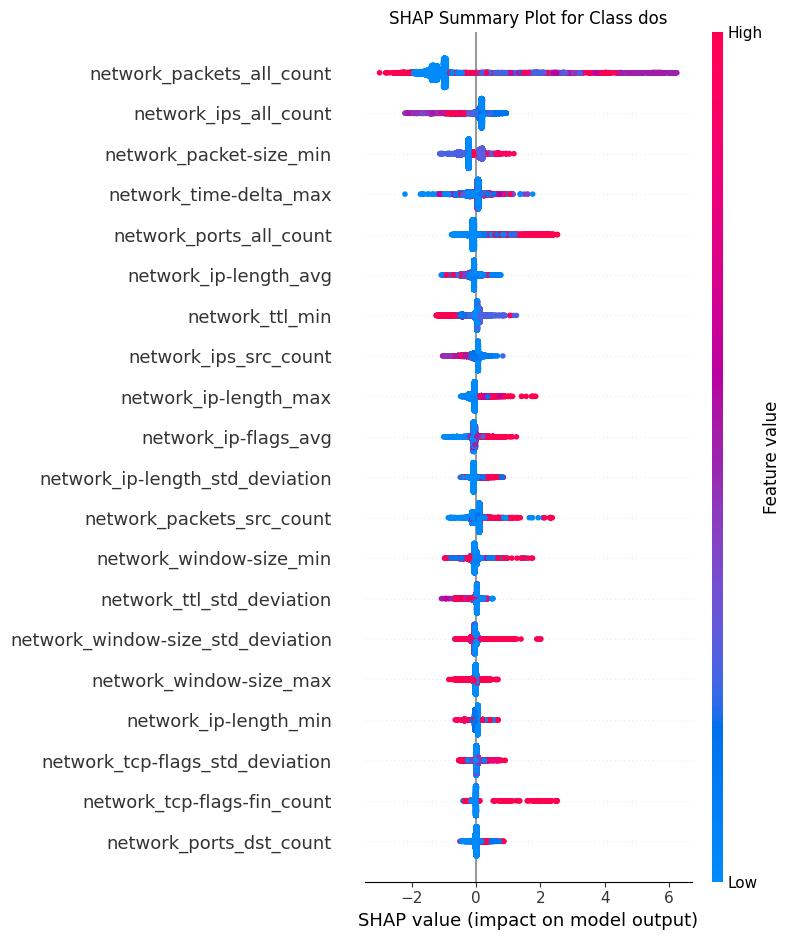
\includegraphics[width=\linewidth]{Images/xai_evaluation/shap_summary_dos.jpeg}}
			{\rule{\linewidth}{2in}}
		\caption{\texttt{dos}}
	\end{subfigure}

	\vspace{0.5em}

	\begin{subfigure}[t]{0.48\textwidth}
		\centering
		\IfFileExists{Images/xai_evaluation/shap_summary_recon.jpeg}
			{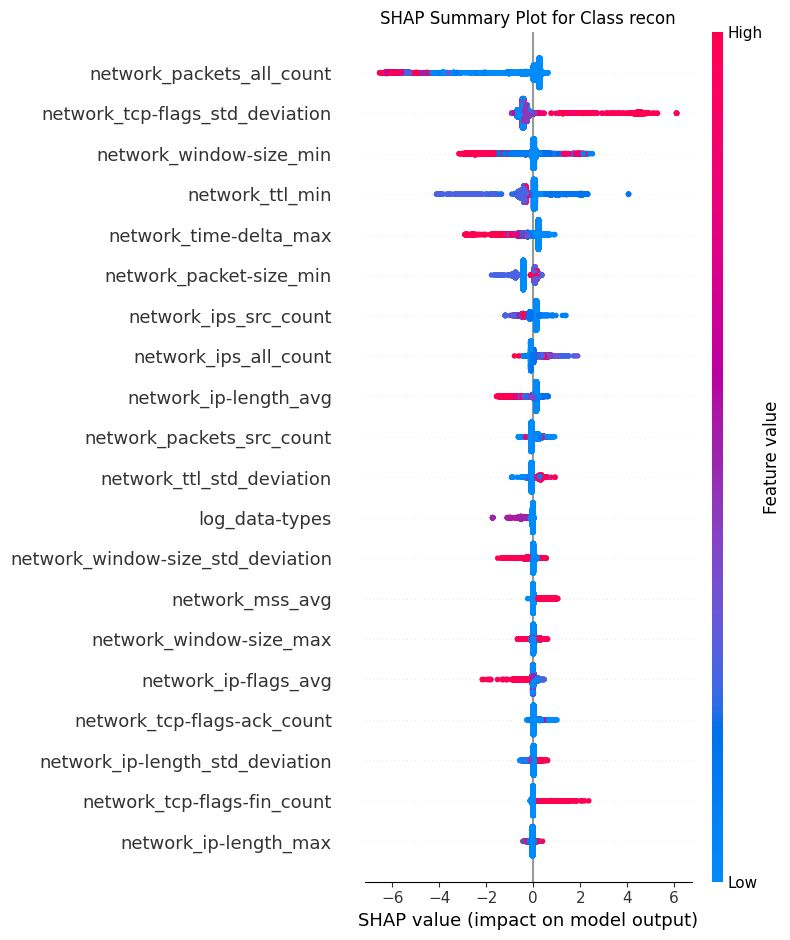
\includegraphics[width=\linewidth]{Images/xai_evaluation/shap_summary_recon.jpeg}}
			{\rule{\linewidth}{2in}}
		\caption{\texttt{recon}}
	\end{subfigure}
	\hfill
	\begin{subfigure}[t]{0.48\textwidth}
		\centering
		\IfFileExists{Images/xai_evaluation/shap_summary_malware.jpeg}
			{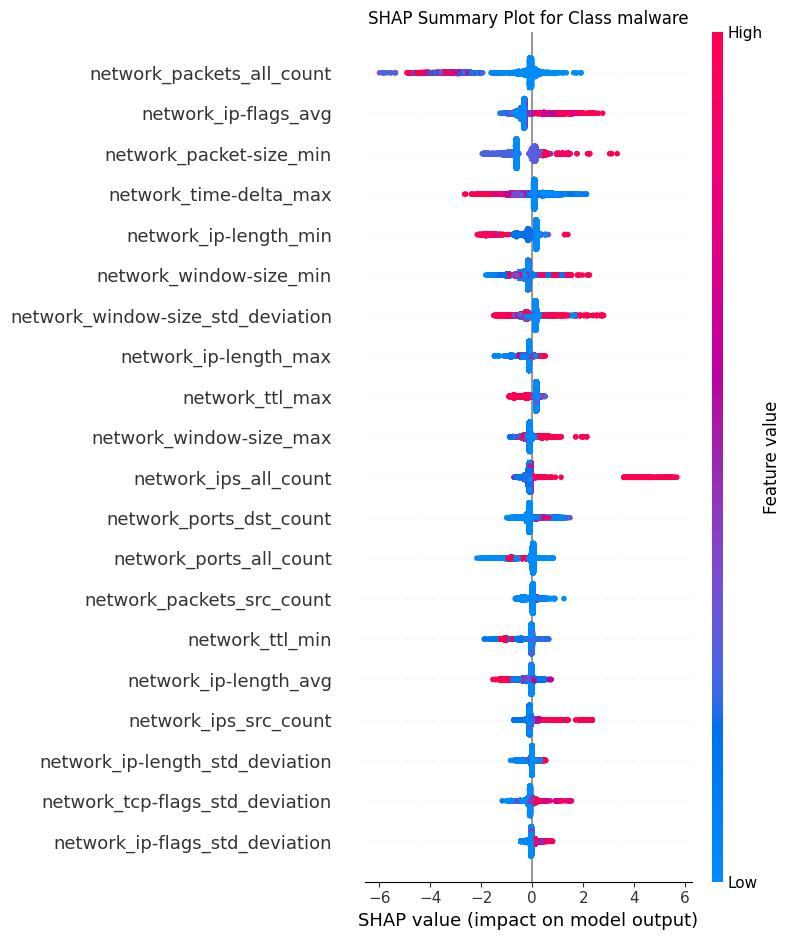
\includegraphics[width=\linewidth]{Images/xai_evaluation/shap_summary_malware.jpeg}}
			{\rule{\linewidth}{2in}}
		\caption{\texttt{malware}}
	\end{subfigure}
	\caption{SHAP summary (beeswarm) plots for the four volume-led attack classes. Long red positive tails on \texttt{network\_packets\_all\_count} across \texttt{ddos}, \texttt{dos}, \texttt{malware}, and \texttt{recon} confirm the shared volume-led direction of those classes.}
	\label{fig:xai_summary_attacks}
\end{figure}

\begin{figure}[htbp]\ContinuedFloat
	\centering
	\begin{subfigure}[t]{0.32\textwidth}
		\centering
		\IfFileExists{Images/xai_evaluation/shap_summary_bruteforce.jpeg}
			{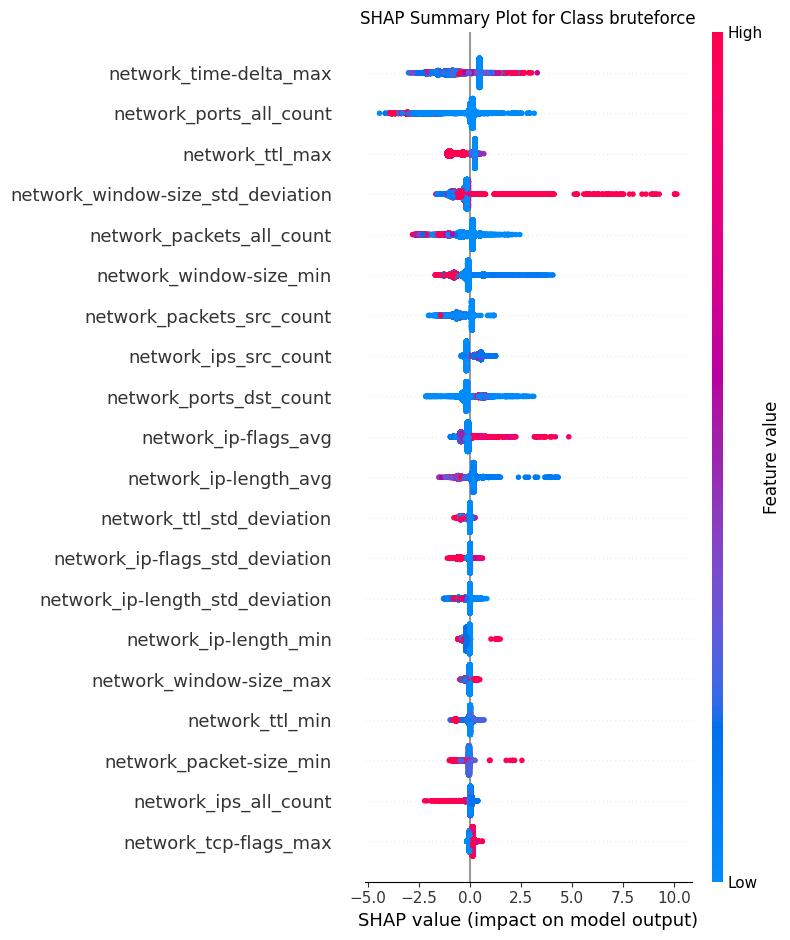
\includegraphics[width=\linewidth]{Images/xai_evaluation/shap_summary_bruteforce.jpeg}}
			{\rule{\linewidth}{2in}}
		\caption{\texttt{bruteforce}}
	\end{subfigure}
	\hfill
	\begin{subfigure}[t]{0.32\textwidth}
		\centering
		\IfFileExists{Images/xai_evaluation/shap_summary_mitm.jpeg}
			{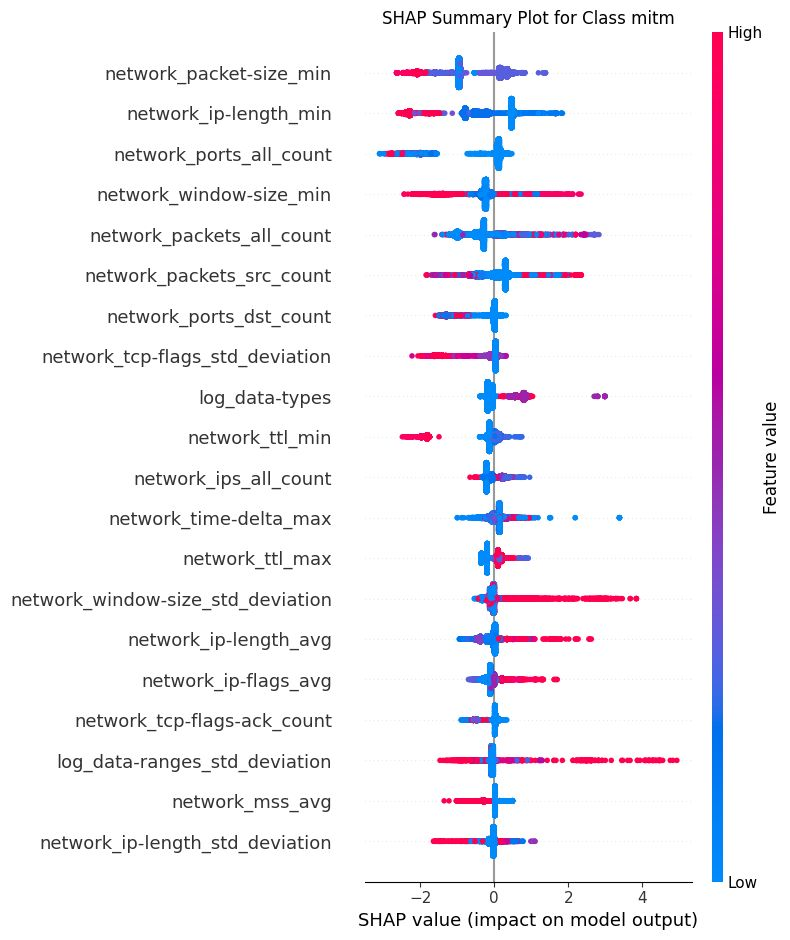
\includegraphics[width=\linewidth]{Images/xai_evaluation/shap_summary_mitm.jpeg}}
			{\rule{\linewidth}{2in}}
		\caption{\texttt{mitm}}
	\end{subfigure}
	\hfill
	\begin{subfigure}[t]{0.32\textwidth}
		\centering
		\IfFileExists{Images/xai_evaluation/shap_summary_web.jpeg}
			{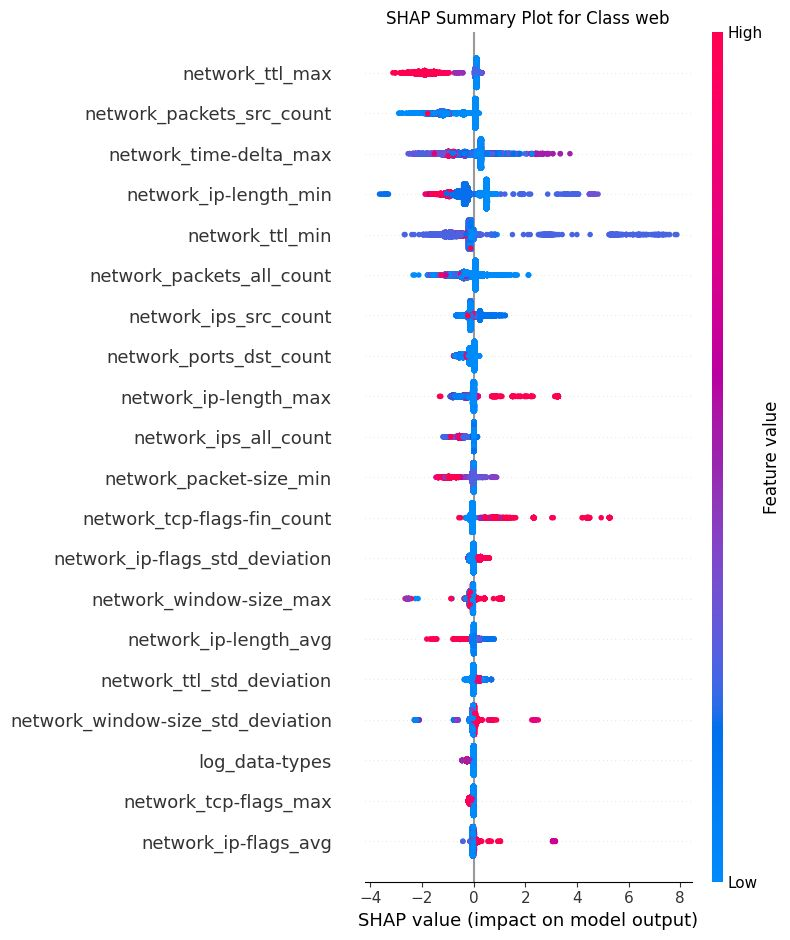
\includegraphics[width=\linewidth]{Images/xai_evaluation/shap_summary_web.jpeg}}
			{\rule{\linewidth}{2in}}
		\caption{\texttt{web}}
	\end{subfigure}
	\caption{SHAP summary (beeswarm) plots for the three distinct-signature attack classes. The visible non-linearity on top-ranked features (particularly for \texttt{mitm}) is the empirical basis for the moderate continuity score reported in Figure \ref{fig:xai_continuity}.}
	\label{fig:xai_summary_attacks_distinct}
\end{figure}

\FloatBarrier

Read together, these metrics indicate that the SHAP subsystem itself is technically sound: attributions are numerically complete, moderately stable, largely contrastive across attack families, and concentrated in a compact head that maps cleanly onto the top-3 statements the healing pipeline ingests. The only two structural concerns they surface, the \texttt{ddos}--\texttt{recon} feature overlap and the leading role of packet-level features in the \texttt{benign} decision, both point at the classifier itself rather than at the explainer, and are consistent with the accuracy findings reported earlier in this section.

\section{Multi-Agent Self-Healing Evaluation}\label{sec:mas_eval}

The true novelty of this framework lies in the autonomous self-healing loop described in Section \ref{sec:multi_agent}: a deterministic ladder engine as the primary decision path, with an LLM consulted only as a fallback. Because the classifier itself is the weak link identified in Section \ref{sec:cloud_eval}, the second round of live testing was deliberately structured to isolate the question of whether the \textit{downstream} mechanics behave correctly \textit{given} a classification that does cross the confidence gate, rather than to report an aggregate end-to-end success percentage that a broken classifier would make meaningless. Each mechanic below was exercised at least once, live, over the full HTTP-driven pipeline, and the outcome recorded as pass or fail rather than as a sampled success rate.

\begin{table}[htbp]
\caption{Self-healing mechanics verified by live, HTTP-driven testing against the full cloud pipeline.}
\label{tb:mas_results}
\centering
\begin{tabular*}{\textwidth}{@{\extracolsep{\fill}}|p{0.22\textwidth}|p{0.54\textwidth}|p{0.14\textwidth}|}
\hline
\textbf{Mechanic} & \textbf{What was exercised} & \textbf{Outcome} \\
\hline
Ladder escalation (P1$\to$P6) & Full \texttt{ddos} playbook escalation driven by simulated edge apply/verification feedback, including a scaled same-level re-apply before advancing to the next tier & Pass \\
\hline
Approval gate at P6 & \texttt{ESC-02} parking the incident in \texttt{pending\_approval}; operator approval correctly dispatching the final action and closing the incident as \texttt{human\_handoff} with an Escalation Agent-authored report & Pass \\
\hline
Benign-state decay & Decay scheduling correctly triggered after a resolution at a ladder level above 0 & Pass \\
\hline
Unhandled-attack routing & An \texttt{unhandled\_attack} classification (no configured ladder) routed directly to the Decision Agent, which retrieved grounded RAG context and selected a coherent action & Pass \\
\hline
Low-confidence-streak trigger & Decision Agent correctly consulted on the second consecutive sub-threshold classification for the same device/attack-type pairing & Pass \\
\hline
Ineffective-LLM-action handling & A Decision Agent action that verification reported as ineffective correctly triggered device isolation (\texttt{SEG-01}) and parked the incident in \texttt{awaiting\_human\_review} until explicitly resolved & Pass \\
\hline
RAG self-learning write-back & Initially found broken for the explicit-verification-feedback path (only the silent no-redetection timeout path worked); confirmed zero \texttt{learned/*.md} entries before the fix and a real entry written after it & Fixed during testing \\
\hline
\end{tabular*}
\end{table}

Every mechanic in Table \ref{tb:mas_results} passed once the classification driving it crossed the confidence gate, which is the central qualitative finding of this evaluation: the resilience-by-design argument of this framework-deterministic ladder, LLM safety net, human handoff, with a human always reachable if every automated tier is exhausted-is validated as engineering, independently of the primary classifier's real-world accuracy. The one mechanic that did not pass on first attempt, RAG self-learning write-back, illustrates why this live-testing methodology was adopted in the first place: a unit-level or code-review check would not necessarily have surfaced that the expected production feedback path (explicit edge verification) bypassed the code that records a successful decision into the retrieval corpus, whereas driving the full loop over HTTP did.

The two grouped buckets noted in Section \ref{sec:cloud_classification} as configured but unreachable, \texttt{lateral\_movement} and \texttt{exfiltration}, could not be exercised by this testing for exactly that reason: no fine-grained label the classifier can currently output maps onto either bucket, so no live classification ever reaches their playbooks. This directly resolves an inconsistency flagged in an earlier draft of this chapter, which reported a \textit{Data Exfiltration} row in this table without a corresponding playbook in Appendix \ref{app:healing_actions}; that row has been removed here, since it described a code path that, as now verified, cannot currently be reached by any classification this system produces. Reconciling the two taxonomies-either by extending the classifier's fine-grained labels to cover exfiltration and lateral-movement patterns, or by removing the two orphaned playbooks until such labels exist-is carried forward as a limitation in Section \ref{sec:limitations_integration} rather than resolved here.

\section{Cloud Dashboard: Operator-Facing Interface}\label{sec:cloud_dashboard}

The cloud tier's evaluation surface, and the intended day-to-day interface for a human operator, is a single-page web dashboard organised into six routes. Every route consumes the same live WebSocket event stream published by the cloud pipeline, so tiles, charts, and log panels all update continuously as new edge-device windows are classified and remediated. This section describes each route in turn, both to document the interface that produced the live findings reported in Sections \ref{sec:edge_eval}--\ref{sec:mas_eval} and to make it clear which parts of the framework are exposed for human oversight and which run without operator involvement.

\subsection{Overview Page}\label{sec:dash_overview}

The Overview page is the default landing route and serves as the executive summary of the entire self-healing pipeline. It is a purely read-only, real-time situational-awareness screen: it does not let the operator take any action but instead aggregates data from every other subsystem (edge ingestion, the XGBoost classifier, the LLM reporting agent, and the healing engine) into a single glanceable view.

Its key UI components are as follows.
\begin{itemize}
	\item Four KPI stat tiles: Devices Monitored (with a currently-under-attack sub-count), Windows Classified (with a flagged-as-attack sub-count), High/Critical Reports, and Healing Actions Issued.
	\item A \textit{Risk timeline} line chart plotting maximum and average classifier confidence in rolling time buckets, giving a temporal view of how risk pressure is trending across the fleet.
	\item A \textit{Severity mix} bar chart summarising LLM report counts across the Low, Medium, High, and Critical bands.
	\item An \textit{Attack type distribution} donut chart summarising XGBoost classification output plus operator and report votes across attack categories (\texttt{benign}, \texttt{ddos}, \texttt{port\_scan}, \texttt{bruteforce}, \texttt{mitm}, \texttt{unhandled\_attack}, and others).
	\item A \textit{Top devices by confidence} ranked table showing device ID, classifier confidence, attack label, severity badge, record count, and last-seen timestamp.
	\item Two live-scrolling event logs shown side by side: \textit{Recent raw ingest} (raw edge windows as they arrive) and \textit{Latest LLM reports} (natural-language incident summaries generated by the reporting LLM agent).
\end{itemize}

\begin{figure}[htbp]
	\begin{center}
		\IfFileExists{Images/cloud/cloud_operations_dashboard.jpeg}
			{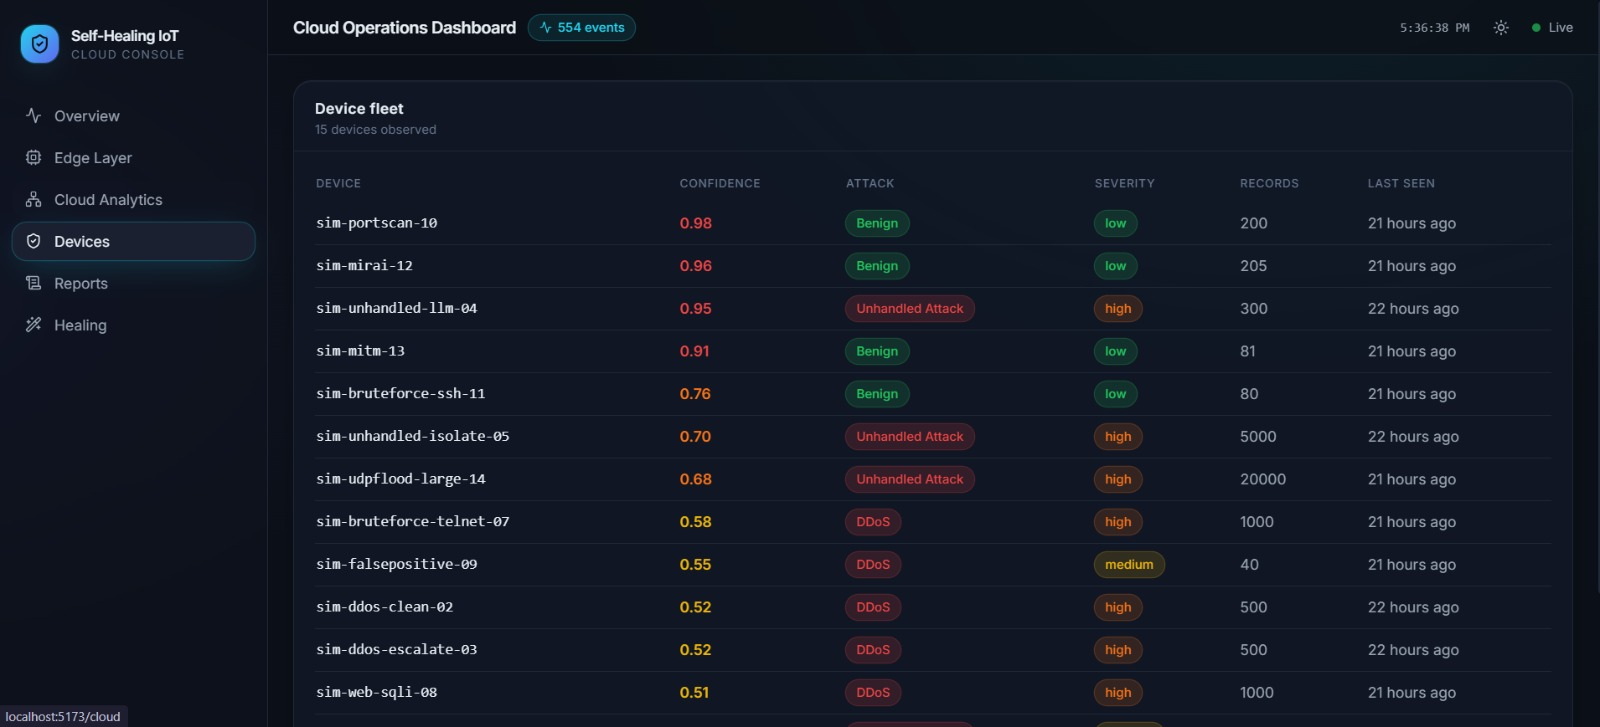
\includegraphics[width=6in]{Images/cloud/cloud_operations_dashboard.jpeg}}
			{\rule{6in}{3.5in}
			\\[-3.7cm]\centering\textit{\small [Image not yet added: Images/cloud/cloud\_operations\_dashboard.jpeg]}\\[3.5in]}
	\end{center}
	\caption{Overview page of the cloud dashboard, aggregating KPI tiles, the risk timeline, severity mix, attack-type distribution, top devices by confidence, and the raw-ingest and LLM-report live feeds into a single situational-awareness view.}
	\label{fig:dash_overview}
\end{figure}

\subsection{Edge Layer Page}\label{sec:dash_edge}

The Edge Layer page narrows the focus to the ingestion boundary of the system, the point at which raw traffic windows are received from simulated or real IoT edge devices and pushed into the XGBoost classifier. Its purpose is to let a developer or researcher validate and stress-test the edge-to-cloud pipeline in isolation, independent of the higher-level healing and reporting logic. It is the only page that contains an interactive traffic-generation control, making it the primary demonstration and testing surface of the dashboard.

Its key UI components are as follows.
\begin{itemize}
	\item Three KPI stat tiles: Raw Windows Received, Attacks Detected, and Average Classification Confidence across the observed fleet.
	\item A \textit{Confidence pressure} timeline chart tracking how the XGBoost classifier's confidence evolves over rolling five-minute windows.
	\item An embedded Edge-Layer Traffic Simulator panel with a Start/Stop control that drives a scripted 15-case test cycle (one simulated device window every approximately two minutes) through the real analytics and healing pipeline end-to-end, together with a \textit{Recent runs} log showing each simulated case as it completes.
	\item A \textit{Raw windows from edge} live log showing the \texttt{POST /api/edge/raw-ingest} payloads as they are received (device ID, record count, window duration, and timestamp).
	\item An \textit{XGBoost classifications} live log shown side by side with the raw feed, displaying the grouped label, the confidence score, and the top SHAP feature-attribution evidence for each classified window.
\end{itemize}

\subsection{Cloud Analytics Page}\label{sec:dash_cloud_analytics}

The Cloud Analytics page is a focused view of the machine-learning classification layer that runs in the cloud tier, distinct from the edge-side metrics on the Edge Layer page. Where the Edge Layer page emphasises ingestion volume and pipeline throughput, this page emphasises classification quality and outcome distribution: it answers ``what is the model finding, and how confident is it?'' rather than ``how much traffic is arriving?''.

Its key UI components are as follows.
\begin{itemize}
	\item Three KPI stat tiles: Classified Windows, Average Classifier Confidence, and Devices Monitored (distinct device IDs seen).
	\item An \textit{Attack type distribution} donut chart summarising the XGBoost classifier's output categories across the observed fleet.
	\item A \textit{Recent classifications} live log listing each classified window with device ID, predicted label and confidence score, and the SHAP feature attributions that explain the model's decision.
\end{itemize}

\begin{figure}[htbp]
	\begin{center}
		\IfFileExists{Images/cloud/cloud_analytics.jpeg}
			{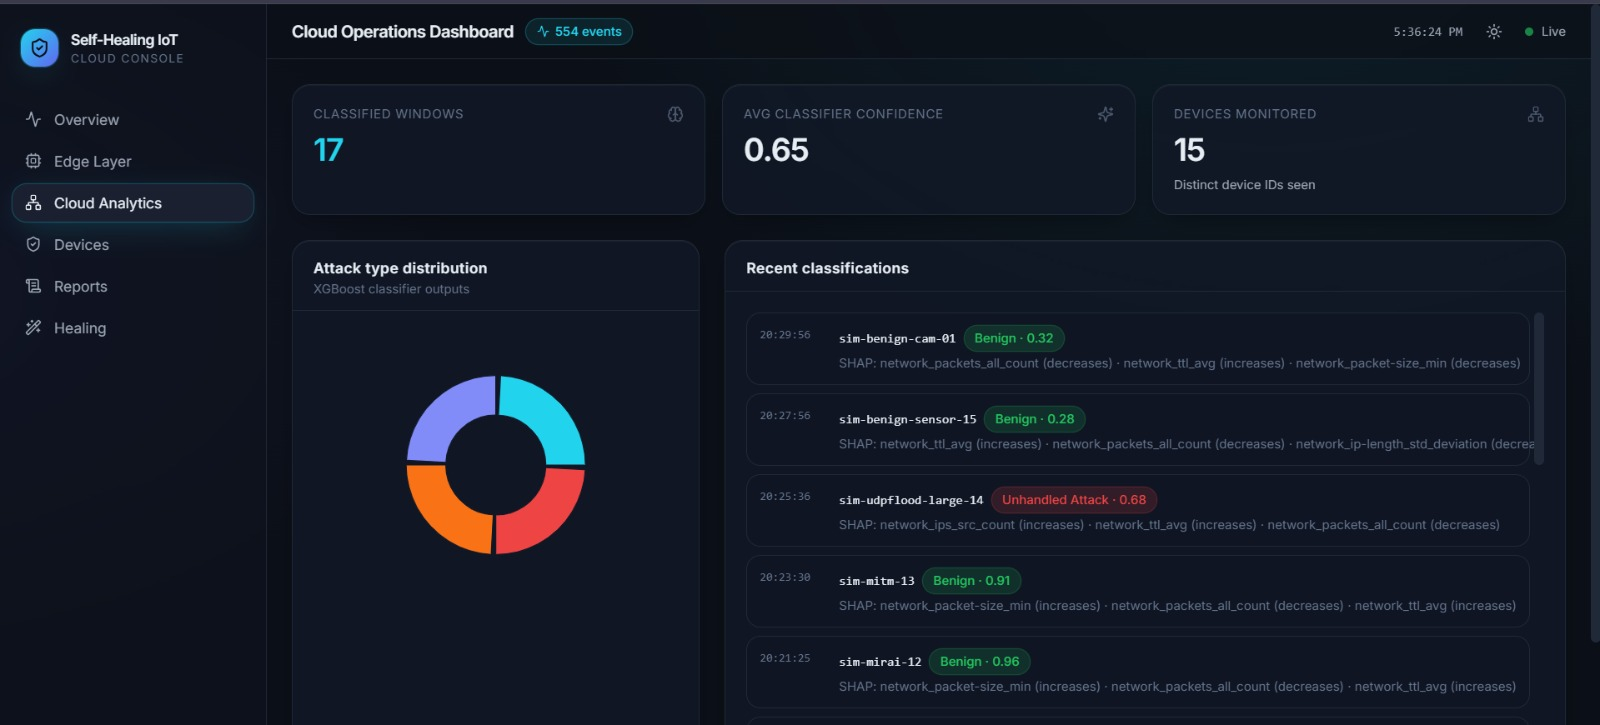
\includegraphics[width=6in]{Images/cloud/cloud_analytics.jpeg}}
			{\rule{6in}{3.5in}
			\\[-3.7cm]\centering\textit{\small [Image not yet added: Images/cloud/cloud\_analytics.jpeg]}\\[3.5in]}
	\end{center}
	\caption{Cloud Analytics page, presenting classifier-side KPIs, the attack-type distribution donut, and the recent-classifications log with per-window SHAP attributions.}
	\label{fig:dash_cloud_analytics}
\end{figure}

\subsection{Devices Page}\label{sec:dash_devices}

The Devices page provides a fleet-inventory view of every IoT device the system has observed, consolidated into a single sortable table rather than split across charts. It is the page an operator would use to look up a specific device's current risk posture, rather than to monitor system-wide trends.

Its key UI components are as follows.
\begin{itemize}
	\item A header showing the total count of observed devices (``Device fleet: $N$ devices observed'').
	\item A full device table (rendering up to 500 rows) with columns for Device ID, Confidence, Attack label (colour-coded, e.g.\ Benign, DDoS, Unhandled Attack), Severity badge (low, medium, or high), Records processed, and Last Seen timestamp.
	\item Rows colour-coded by risk: confidence values shift from green (low risk) through amber to red (high risk), and severity badges use the same low/medium/high colour language used throughout the rest of the dashboard for visual consistency.
\end{itemize}

\subsection{Reports Page}\label{sec:dash_reports}

The Reports page exposes the output of the LLM-based security reporting agent: every classified incident is summarised by the LLM into a structured natural-language report with recommended actions, and this page lets an operator browse and drill into that report history. It follows a master--detail interaction pattern, which distinguishes it from the purely passive log views on the Overview and Cloud Analytics pages.

Its key UI components are as follows.
\begin{itemize}
	\item Left panel: a scrollable, clickable list of \textit{LLM security reports}, each row showing device ID, a severity badge (low, medium, or high), the attack label, and the report timestamp.
	\item Right panel: the detail view for the selected report, showing a one-line natural-language summary; a badge row (severity, confidence score, and source engine, for example \texttt{mock} or \texttt{llm}); an \textit{Indicators} section listing the SHAP-derived signals that drove the classification (feature name, direction of influence, and SHAP value); a \textit{Recommended actions} panel with the suggested remediation, its category tag (for example \texttt{observation}), and rationale; and a raw JSON \textit{Evidence} viewer exposing the full underlying model output for auditability.
	\item User interaction: clicking any report in the left list refreshes the right-hand detail panel. This is the only page besides Healing where the user actively selects an item to inspect rather than only observing a live feed.
\end{itemize}

\begin{figure}[htbp]
	\begin{center}
		\IfFileExists{Images/cloud/reports_page.jpeg}
			{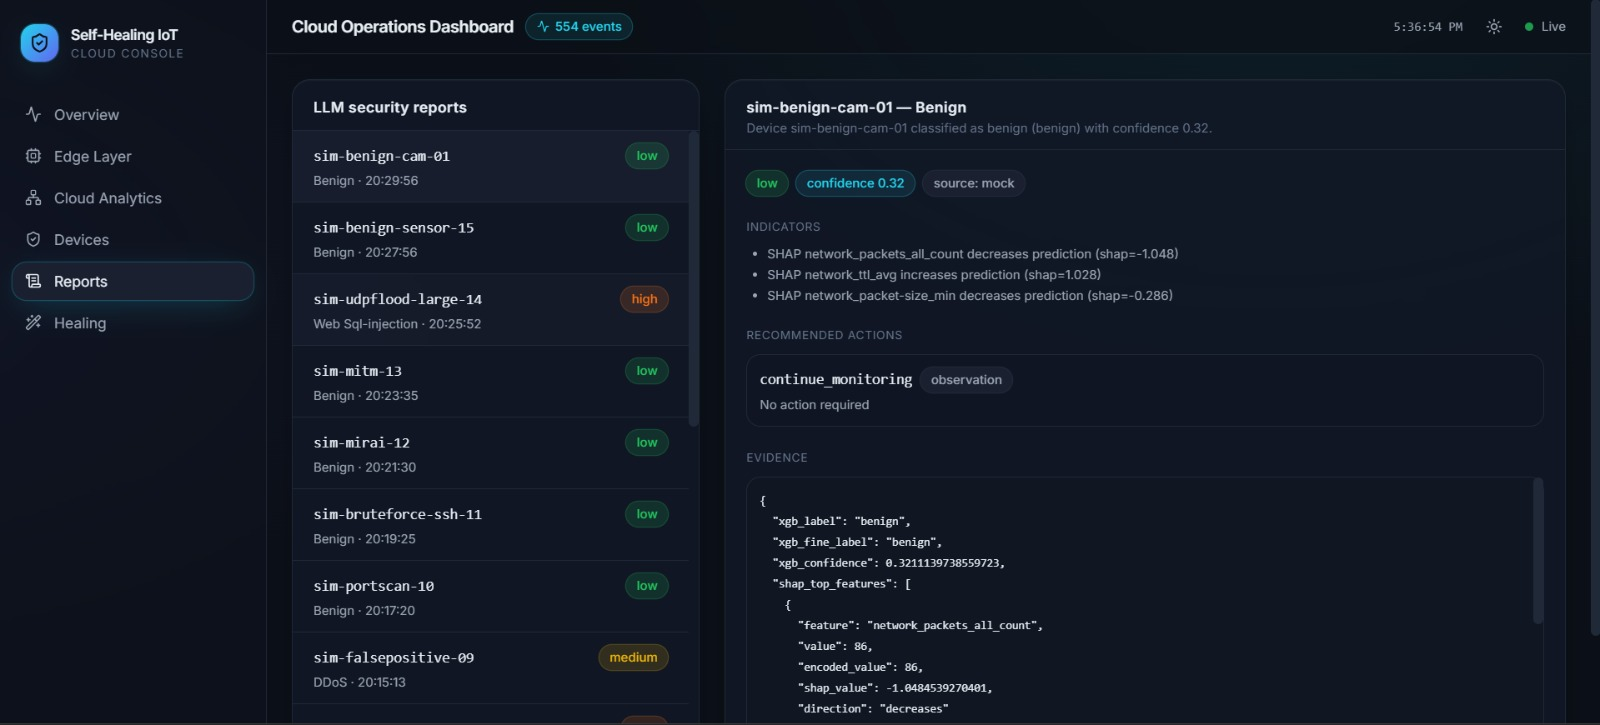
\includegraphics[width=6in]{Images/cloud/reports_page.jpeg}}
			{\rule{6in}{3.5in}
			\\[-3.7cm]\centering\textit{\small [Image not yet added: Images/cloud/reports\_page.jpeg]}\\[3.5in]}
	\end{center}
	\caption{Reports page, showing the master list of LLM-generated security reports on the left and the selected report's detail view (summary, indicators, recommended actions, and raw evidence JSON) on the right.}
	\label{fig:dash_reports}
\end{figure}

\subsection{Healing Page}\label{sec:dash_healing}

The Healing page is the operational core of the self-healing system and the most interactive page in the application. It visualises the automated incident-response workflow: a deterministic escalation ladder (P1 to P6 for network-layer responses, or B0 to B4 for device-layer responses) that attempts increasingly aggressive remediation actions, escalating to an LLM-based Decision Agent (grounded via Retrieval-Augmented Generation over a knowledge base of prior playbooks) when the deterministic ladder is exhausted or confidence is low, and finally isolating a device and handing it to a human operator when neither can resolve the incident with confidence. This page is where human-in-the-loop review and approval actually happens.

Its key UI components are as follows.
\begin{itemize}
	\item \textit{Active incidents} panel: incidents currently being remediated, each rendered as a card with status, attack-type, and device badges, and a chronological timeline of remediation attempts (ladder level, action taken, outcome, and whether the action ran in dry-run or audit mode).
	\item \textit{Resolved and handed-off} panel: closed incidents that fed back into the incident-memory store, shown with the same timeline format plus a final outcome badge (Resolved, Isolated, or Human handoff) and the resolution source (for example \texttt{via edge\_confirmed} or \texttt{via manual\_isolation\_released}).
	\item Decision Agent notes: rendered inline in an incident's timeline whenever the deterministic ladder escalates to the LLM, shown as a highlighted card with the trigger reason (for example \texttt{ladder exhausted} or \texttt{low-confidence streak}), a RAG-grounded tag, the chosen action code, a confidence percentage, and the agent's natural-language rationale for the decision.
	\item Approval Actions widget: Approve and Reject buttons shown on incidents awaiting operator sign-off before a remediation action is applied (wired to \texttt{api.approveIncident} and \texttt{api.rejectIncident}).
	\item Human Review Actions widget: for devices that have been isolated and require a human decision, three buttons are offered: \textit{Release isolation and resolve}, \textit{Handled manually}, and \textit{Escalate to permanent quarantine} (wired to \texttt{api.\allowbreak resolveHumanReview}).
	\item Operator Brief: a summary and recommendation box shown on handed-off incidents, generated by the LLM handoff agent to brief the human reviewer on what happened, what was tried, and what is recommended next (including a suggested follow-up action code).
\end{itemize}

\begin{figure}[htbp]
	\begin{center}
		\IfFileExists{Images/cloud/healing_page.jpeg}
			{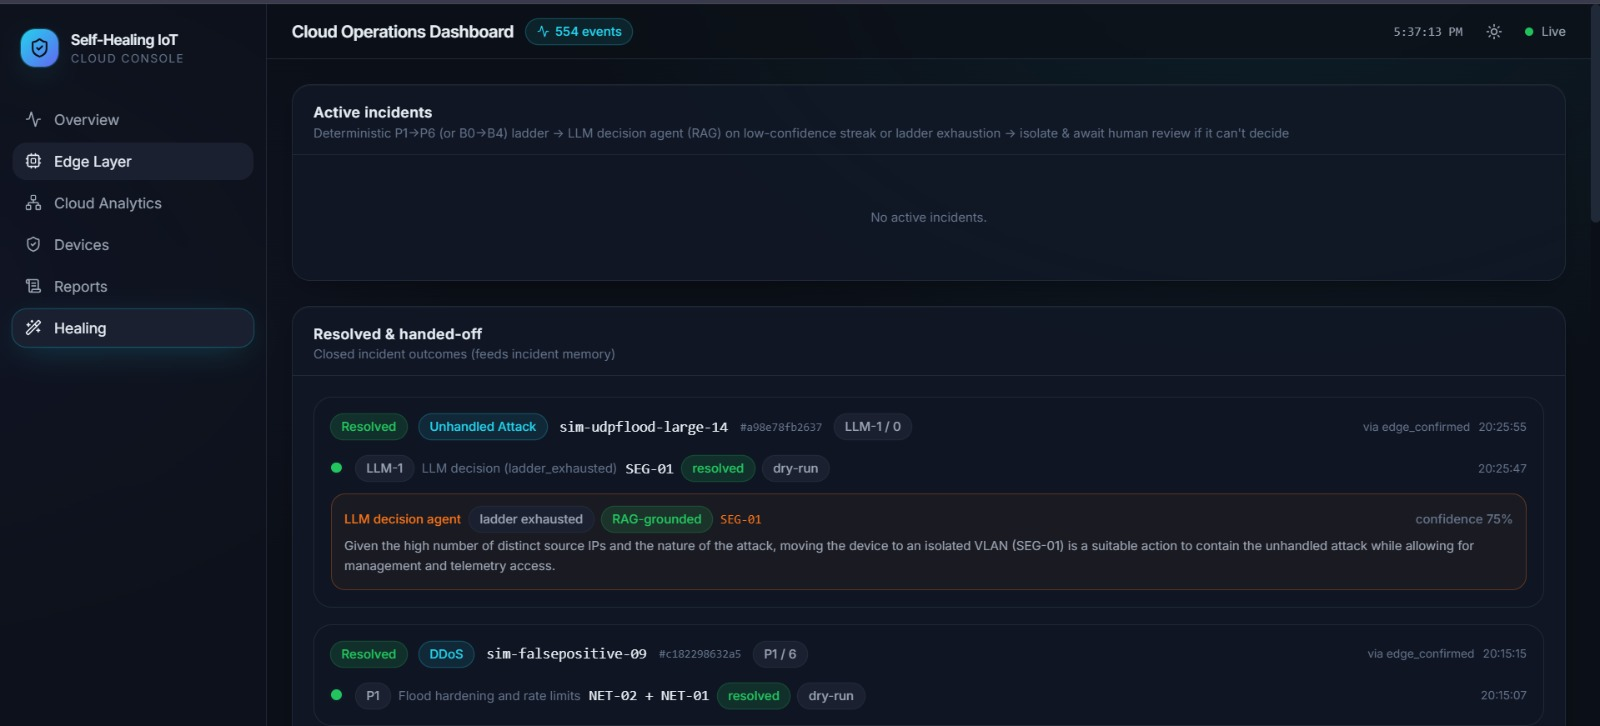
\includegraphics[width=6in]{Images/cloud/healing_page.jpeg}}
			{\rule{6in}{3.5in}
			\\[-3.7cm]\centering\textit{\small [Image not yet added: Images/cloud/healing\_page.jpeg]}\\[3.5in]}
	\end{center}
	\caption{Healing page, showing the active and resolved incident panels, inline Decision Agent notes, the approval and human-review widgets, and the LLM-generated Operator Brief on handed-off incidents.}
	\label{fig:dash_healing}
\end{figure}

\FloatBarrier

\section{Discussion}

The experimental results validate the core hypothesis of this research: a distributed, multi-stage architecture can successfully bridge the gap between lightweight anomaly detection and heavy, cognitive incident remediation in IoT networks.

\subsection{Edge Intelligence and the Mitigation of Alert Fatigue}
The superior performance of the Cascaded Hybrid Ensemble (F1-Score of 0.9971, Table \ref{tb:edge_results}) underscores the necessity of temporal awareness in IoT security. Standard static models, including the standalone Isolation Forest and standalone Deep SVDD baselines, both misclassify benign, bursty IoT telemetry as anomalous considerably more often than the fused ensemble, with standalone Deep SVDD in particular exhibiting a precision of only 53.3\% despite a comparable recall-consistent with a model that flags a great deal of benign traffic while still catching most attacks. By leveraging the GRU autoencoder to extract temporal embeddings via RMSprop optimization, the ensemble successfully captures the sequential state of the network before applying the Deep SVDD boundary. Furthermore, the Two-Stage Rolling Risk Score proved highly effective in practice. In production-like environments, security operations centers (SOCs) are often overwhelmed by transient network spikes. The rolling score acts as a low-pass filter, mathematically isolating sustained, systematic attacks from benign network jitter, effectively solving the alert fatigue problem at the edge. As discussed in Section \ref{sec:cloud_classification}, this edge-side mechanism currently operates independently of the cloud tier rather than gating what the cloud receives; Section \ref{sec:limitations_integration} discusses why.

\subsection{The Paradigm Shift to Machine-Readable XAI}
Traditionally, XAI frameworks like SHAP are designed as visualization tools for human analysts. A critical design choice in this framework is pivoting XAI to serve as a machine-to-machine interface as well: the same translated SHAP attributions that populate the Dashboard Reporting Agent's operator-facing summaries are also inserted into the prompt whenever the Decision Agent or Escalation Agent is consulted (Section \ref{sec:multi_agent}), rather than maintaining a separate, human-only explanation path. This enables whichever LLM component is invoked to reason over the specific network features that drove a classification, rather than the classification label alone, allowing for a more targeted fallback decision than a blunt default action would be. This benefit is, however, only as good as the classification being explained; Section \ref{sec:cloud_eval}'s findings on classifier accuracy apply equally to what the explainer is explaining.

\subsection{Autonomous Remediation and System Limitations}\label{sec:limitations_integration}
The multi-agent RAG pipeline demonstrated correct behaviour, mechanic by mechanic, in dynamically issuing and escalating healing commands once given a classification to act on (Table \ref{tb:mas_results}). The use of a RAG architecture successfully constrained the LLM fallback agents' outputs to physically viable commands drawn from the catalogue in Appendix \ref{app:healing_actions}, rather than free-composing network configurations that might not exist on the target device.

However, live verification testing surfaced limitations considerably more specific, and in places more serious, than could be identified from the architecture alone:

\begin{enumerate}
	\item \textbf{Classifier accuracy on real-world traffic is the framework's primary weakness, not the surrounding engineering.} Section \ref{sec:cloud_eval} documents false negatives at 90--98\% confidence, false positives that dispatched real containment against a benign device, non-monotonic confidence with attack volume, and frequently incorrect fine-grained labels even when the grouped bucket's gate is crossed. The root cause is a granularity mismatch: the classifier was trained on packet-level captures, and roughly half of its expected input features are permanently placeholder-filled because the edge layer forwards connection-log aggregates rather than packet captures. No amount of improvement to the ladder engine, the RAG grounding, or the LLM fallback agents corrects a decision made on a classification that was wrong to begin with; closing this gap requires either retraining the classifier on connection-log-derived features directly, or upgrading the edge layer's telemetry to genuinely supply the packet-level signals the current model expects.
	\item \textbf{Two of the eight configured healing playbooks are currently dead code.} \texttt{lateral\_movement} and \texttt{exfiltration} each have a full prioritised playbook in Appendix \ref{app:healing_actions}, but no fine-grained label the classifier produces maps onto either grouped bucket, so neither playbook can currently be triggered by any classification this system makes. As noted in Section \ref{sec:hybrid_ensemble}, this is at least partly explained by the training data itself: the CIC IIoT 2025 dataset's native taxonomy of 50 attack types spans seven categories (DDoS, DoS, Reconnaissance, Web, Bruteforce, MITM, and Malware/Mirai) that do not include either lateral movement or exfiltration as a category \cite{Firouzi2025}, so a classifier trained to discriminate that taxonomy has no basis for ever emitting a label that would route to either bucket. This was surfaced by, rather than hidden by, the verification process, and is recorded here as an open item rather than corrected silently.
	\item \textbf{Reliance on large cloud-based LLM APIs introduces API latency and recurring computational costs}, which may not be scalable for massively distributed micro-networks without optimization, and which is a further reason the ladder engine, rather than an LLM, is the primary decision path (Section \ref{sec:multi_agent}) rather than a secondary optimisation.
	\item \textbf{The cognitive cloud tier inherently relies on the availability of the edge-to-cloud communication link} once that link exists in a deployed sense. While the edge layer is designed to reserve bandwidth for this telemetry, a severe, distributed link-flooding attack could theoretically isolate the edge node before any healing action reaches it.
\end{enumerate}


%%%%%%%%%%%%%%%%%%%%%%%%%%%%%%%%%%%%%%%%%%%%%%%%%%%%%%%%%%%%%%%%%%%%%%%%%%%%%%%%%%%%%%%%%%%%%%%%%%
%%%%%%%%%%% END OF FILE
%%%%%%%%%%%%%%%%%%%%%%%%%%%%%%%%%%%%%%%%%%%%%%%%%%%%%%%%%%%%%%%%%%%%%%%%%%%%%%%%%%%%%%%%%%%%%%%%%%